%|============================================================================|
%| Bachelor Arbeit Frederik Eberhard am Institut ieet                         |
%|============================================================================|

% ---- Definition der Dokumenteneigenschaften ----
\documentclass[
              11pt,								  % Schriftgröße
              twoside,                              % Beidseitig (für einseiteig "oneside"')
              numbers=noenddot,                     % Kapitelnummern etc. haben keinen "Endpunkt", vorher Kap. 2.2., jetzt Kap. 2.2
              listof=totoc,                         % Fügt Abbildungs- und Tabellenverzeichnis zum Inhaltsverzeichnis zu
              bibliography=totoc,                   % Fügt das Literaturverzeichnis zum Inhaltsverzeichnis zu
              captions=tableheading, % Stellt den Abstand zwischen Tabellenüberschrift her, sonst einfach mit \captionabove
              %parskip=half-                        % Absätze werden durch einen vertikalen Abstand von einer halben Zeile gekennzeichnet. Absatzenden werden nicht gekennzeichnet.
              openright,							% Kapitel werden bei beidseitigem Druck rechts begonnen
              ]{scrreprt}                           % KOMA-Klasse für "report" (BA/MA/Dipl.-Arbeiten)
% !TeX root =../main.tex
%Bitte hier die Daten anpassen

\newcommand{\MScBSc}{0} % 0=Bachelorarbeit 1=Projektarbeit 2=Masterarbeit
\newcommand{\Sprache}{1} % 0=Deutsch 1=Englisch 
% Wenn die Sprache geändert wird muss eventuell zweimal kompiliert werden um eine auftretende Fehlermeldung zu beheben.

\newcommand{\MitDanksagung}{0} % 0 = Nein, 1 = Ja, die Danksagung ist optional

\newcommand{\VornameDesStudenten}{Frederik}
\newcommand{\NachnameDesStudenten}{Eberhard}
\newcommand{\Matrikelnummer}{521446}
\newcommand{\Studiengang}{Student der Elektrotechnik} %{M.Sc. Elektrotechnik / ETMS} %bitte in diesem Stil lassen!
\newcommand{\BetreuerE}{Thomas William Walsh}
\newcommand{\BetreuerZ}{Leon Maximilian Helmich} % Nur falls einen zweiten Betreuer gibt ändern, sonst unveränert lassen
\newcommand{\IEETNumber}{24.033} % {Num} durch Nummer der Arbeit ersetzen 
\newcommand{\Abgabe}{September 2024}
\newcommand{\Zweitpruefer}{Zweitprüfer} % Nur bei Masterarbeiten einzutragen
\newcommand{\Ort}{Harburg} % Bitte Wohnort eintragen
%Hier den Titel der Arbeit eintragen
\newcommand{\DeutscherTitelDerArbeit}{
		  \large
          \normalfont \bfseries
           Schätzung der AC- und DC-Verluste in den Induktivitäten eines Schaltnetzteils\\
          }
\newcommand{\EnglischerTitelDerArbeit}{
	\small %normalsize
	\normalfont \bfseries
    Estimating AC and DC losses in the inductors of a switch mode power supply\\
}

% Hier braucht keine Änderung vorgenommen werden.
\newcommand{\ArtDerArbeit}{\ifthenelse{\equal{\MScBSc}{0}}
			{\ifthenelse{\equal{\Sprache}{0}}
				{Bachelorarbeit}{}
			\ifthenelse{\equal{\Sprache}{1}}
			{Bachelor's Thesis}{}}
		{\ifthenelse{\equal{\MScBSc}{1}}
			{\ifthenelse{\equal{\Sprache}{0}}
				{Projektarbeit}{}
				\ifthenelse{\equal{\Sprache}{1}}
				{Project Thesis}{}
			}{}
		\ifthenelse{\equal{\MScBSc}{2}}
			{\ifthenelse{\equal{\Sprache}{0}}
				{{Masterarbeit}}{}
				\ifthenelse{\equal{\Sprache}{1}}
				{{Master's Thesis}}{}
			}{}}}
	
%|============================================================================|
%| Pakete und Einstellungen                                                   |
%|============================================================================|

% ---- Eigene Packages----
\usepackage[colorinlistoftodos]{todonotes}
% ------------------------

\usepackage{ifthen}

% ---- Spracheinstellungen ----
%\usepackage[ngerman]{babel}		% Neue dt. Rechtschreibung, Silbentrennung (auch im Literaturverzeichnis)
\ifthenelse{\equal{\Sprache}{0}}
	{\usepackage[ngerman]{babel}
	\usepackage[ngerman]{isodate}
     \usepackage{ziffer} % Stellt sicher, dass im Deutschen keine Spaces zwischen Kommas in Zahlen vorkommen (1, 155 wird 1,155}
	}{}
\ifthenelse{\equal{\Sprache}{1}}
	{\usepackage[ngerman,english]{babel}
	\usepackage[ngerman,english]{isodate}
	}{}


\usepackage[utf8]{inputenc}		% Deutsche Sonderzeichen/ Umlaute
\usepackage{helvet}             % Schriftart Helvetiva
% Schriftart Helvetica für Überschriften und Text
\renewcommand\familydefault{phv}
\usepackage{csquotes}
\usepackage[T1]{fontenc}        % Stellt sicher, dass im PDF Umlaute gefunden werden
\usepackage{textcomp}           % Zusätzliche Symbole
\usepackage{setspace}
\setlength{\emergencystretch}{2em}		% erlaubt größeren Leerraum zwischen Wörtern, damit bei Blocksatz besser umgebrochen werden kann (reduziert overfull\hbx-Meldungen)
%In diesem Package lassen sich Silbentrennungen für Zeilenumbrüche von unbekannten Wörtern definieren
\hyphenchar\font=\string"7F
\hyphenation{Wirk-leis-tungs-un-gleich-ge-wicht Mo-men-tan-re-ser-ve}					


% ---- Mathe, Physik etc. ----
\usepackage[
            fleqn                                     % Linksbündige Formeln
            ]{amsmath}                                % Zur Abbildung der mathematischen Symbole und Formeln
\usepackage[fixamsmath,disallowspaces]{mathtools}     % Erweitert amsmath und behebt einige Fehler
\usepackage{nccmath}
\usepackage{amsfonts}                                 % Mathematische Schriftarten
\usepackage{array} 									  % array-Umgebung (für Matrizen etc)
\usepackage{bm} 		% Fett schreiben im Mathemodus über \bm
%\sisetup{locale = DE}
\usepackage{siunitx}	% sorgt für eine korrekte Darstellung von Einheiten; Umwandlung in andere Systeme als SI möglich
%\usepackage{ziffer}   	% Verhindert den kleinen Platz nach Kommas im Mathemodus
\ifthenelse{\equal{\Sprache}{0}}{\sisetup{locale = DE}}{\sisetup{locale = EN}}


% ---- Kopfzeile ----
% Seitenstil, verhindert nur Großbuchstaben im Header, "plainheadsepline" erstellt auch eine Linie bei Chapter
\usepackage[automark, plainheadsepline, headsepline]{scrlayer-scrpage}


% ---- Abbildungen ----
\usepackage[
           singlelinecheck=false,	% Linksbündige Captions
           labelfont=bf
           ]
           {caption}[2008/08/24]	% Erzeugt eine numerierte Bemerkung innerhalb der figure- und table-Umgebungen
\usepackage{subcaption}				% Captions für Unterbilder
\usepackage{graphicx,psfrag}        % Einbindung von Abbildungen, EPS Benutzung
\usepackage{flafter} 				% Verhindert, dass eine Abbildung im Text vor der ersten Nennung auftaucht
																																		 

\usepackage{here}       % Zum erzwingen der Bildplatzierung mit [H] (am besten nicht erzwingen sondern fließen lassen und nur machen wenn der satzspiegel einer Seite gut ist!!)
\usepackage{epstopdf}   % Wandelt *.eps-Dateien on the fly in PDF´s um, damit die Konvertierung direkt in PDF klappt


% ---- Gleitparamter für optimales Gleiten von Abb. und Tab. ----
\setcounter{topnumber}               {1}
    \setcounter{bottomnumber}        {1}
    \renewcommand{\floatpagefraction}{0.8}
    \renewcommand{\topfraction}      {0.8}
    \renewcommand{\bottomfraction}   {0.5}
    \renewcommand{\textfraction}     {0.15}
    \makeatletter
      \setlength{\@fptop}{0pt}
    \makeatother

	
% ---- Fussnoten ----
\usepackage{chngcntr}             	% Erlaubt das Erstellen und Ändern eigener Counter
\counterwithout{footnote}{chapter}  % Lässt die Nummerierung der Fußnoten auch über Kapitel hinweg fortlaufen, wenn nach jedem neuen Kapitel bei 1 angefangen werden soll -> auskomemntieren
\usepackage{footmisc}               % Fußote eingerückt, in der nächsten Zeile wieder linksbündig0


% ---- ANHANG ----
\usepackage[toc,page,title,header]{appendix} 			%toc: Anhang wird im Inhaltsverzeichnis gezeigt
\addto\captionsngerman{\let\appendixtocname\appendixname
\let\appendixpagename\appendixname} 					%Das deutsche Wort Anhang wird statt Appendix angezeigt


% ---- Abkürzungen ----
\usepackage{acronym} % Abkürzungen werden in der Datei 'abkuerzungen.tex' definiert
% \acro{Kurzname}{Langname} in der Umgebung \begin{acronym} (s. Datei)
% Bsp.: \acro{WKA}{Windkraftanlage}
% Im Text schreibt man statt 'WKA' '\ac{WKA}'. An der Stelle des ersten Aurufs steht
% automatisch Windkraftanlage (WKA) und ab da an nur noch WKA
% Der Plural von Abkürzungen wird mit \acp aufgerufen. Wenn der Plural des Wortes nicht
% durch ein 's' erzeugt wird (englisches Package) muss er gesondert definiert werden
% \acrodefplural{WKA}[WKA]{Windkraftanlagen} - der Plural von WKA wird hier ebenfalls mit WKA
% abgekürzt.


% ---- Verwaiste Zeilen ----
\usepackage[all]{nowidow}	% Verhindert, dass eine einzelne Zeile (Waisenzeile) am Ende einer Seite (nach einem Absatz), bzw. am Anfang einer Seite (zum Ende eines Absatzes) auftaucht

% ---- TABELLEN ----
\usepackage{color}					% für Farben im allgemeinen
\usepackage{colortbl}				% für die Hintergrundfarbe einzelner Zellen in Tabellen
\usepackage{multirow}				% Erlaubt es, innerhalb einer Tabelle mehrzeilige/spaltige Zellen zu erstellen
\usepackage{rotating}				% Schrift in Tabellen vertikal ausrichten durch \begin{sideways} TEXT \end{sideways}
\usepackage{tabularx} 				% Tabellen mit variabel breiten Spalten (gekennzeichnet durch X), so dass die Tabelle immer auf die Breite der Seite gestreckt wird
\usepackage{xltabular}              % Tabellen brechen selbstständig und verlaufen über mehrere Seiten

% ---- LITERATURVERZEICHNIS ----
% Das Literaturverzeichnis wird über biblatex mit dem Backend biber erstellt.
% Die Literatur wird in der Datei literatur.bib abgelget, die bspw. mit JabRef bearbeitet werden kann
% Um die Datei richtig kompilieren zu können, muss die Art der Bibliographie (Biblographie->Art) auf biblatex gestellt sein
% Außerdem muss unter (Optionen->Texstudio konfigurieren->Erzeugen) das Standard Bibliographieprogramm auf 'Biber' gestellt sein.
% In anderen Latex-Umgebungen sollten sich ähnliche Einstellungen finden lassen

% \usepackage[backend=biber,  	% Das Backend zum kompilieren der .bib-Datei
% 			style=ieee, 		% Der Stil indem das Literaturverzeichnis angezeigt wird
% 			citestyle=numeric,
% 			urldate =comp] 	% Zitate im Text werden durchnumeriert und entsprechend im Verzeichnis geordnet
% 			{biblatex}
% \renewbibmacro*{author}{\printnames{author}} % Verhindert, dass gleiche Autorennamen hintereinander durch Striche ersetzt werden (ist im ieee-Style implementiert)

%\addbibresource{Literatur/literatur.bib} % Pfad zur .bib-Datei


% ---- Farbdefinitionen ----
\definecolor{dunkelgrau}{rgb}{0.8,0.8,0.8}
\definecolor{hellgrau}{rgb}{0.95,0.95,0.95}
\definecolor{hellblau}{rgb}{0.8,0.8,0.8}


% ---- DIVERSES ----
\usepackage{pdfpages}		% PDF-Seiten im Anhang einbinden
\raggedbottom				% SOLL BEI TWOSIDED VERHINDERN DASS ABSTÄNDE ZU GROß SIND
\usepackage{tikz}
\usetikzlibrary{positioning}
\usetikzlibrary{pgfplots.groupplots}
\usetikzlibrary{patterns} %for patterns in bar plot
\usetikzlibrary{spy}
\usepackage{amssymb}
% ======================== Optionale Pakete ===========================
% an dieser Stelle können eigene Pakete eingebunden werden.
% bereits vorhandene Pakete können bei Bedarf einkommentiert werden

%\usepackage[official]{eurosym}  % Offizielles Euro-Zeichen

%\usepackage{multirow}			 % Erlaubt es, innerhalb einer Tabelle mehrzeilige/spaltige Zellen zu erstellen

%\usepackage{colortbl}   		 % Tabellellinien in anderen Farben

%\usepackage{overpic}			 % Bilder mit anderen Bildern überlagern (Bspw. für Legenden)

%\usepackage{pdflscape}		     % einzelne Seite im Querformat

%\usepackage{listings}					% Führt Listings zur Darstellung von Code ein					
%\renewcommand{\lstlistingname}{Programmcode}	% Ändert Titel der Listings

\usepackage{pgfplots} % TICKZ einbinden (PGF)
\pgfplotsset{compat=1.18}
\usepackage{algorithm}	% Include Pseudocode, algorithmic
\usepackage{algpseudocode}

\ifthenelse{\equal{\Sprache}{0}}
	{% Abbildung
	\newcommand{\figref}[1]{Abb.~\ref{#1}}
	% Gleichungs--Referenzen:
	\renewcommand{\eqref}[1]{Gl.~(\ref{#1})}
	}{}
\ifthenelse{\equal{\Sprache}{1}}
{% Abbildung
	\newcommand{\figref}[1]{Fig.~\ref{#1}}
	% Gleichungs--Referenzen:
	\renewcommand{\eqref}[1]{Eq.~(\ref{#1})}
}{}
\newcommand{\tabref}[1]{Tab.~\ref{#1}}
% Algorithmus --Referenzen: 
\newcommand{\algoref}[1]{Alg.~\ref{#1}}
% ==================================================================


% ---- HYPERREF ---- !WICHTIG! - {hyperref} als letztes Paket laden
\usepackage{hyperref}	% Verlinkung von farbigen Referenzen im Text, z.B. Verlinkung direkt zu einer Fußnote oder Literatur
\hypersetup{
  colorlinks=true,	% aktiviert farbige Referenzen
  linkcolor=black,	% Farbe der Verlinkungen innerhalb des Textes, z.B. Kapitel, Fußnote etc.
  citecolor=black,	% Farbe der Literatur-Refs
  urlcolor=black,	% Farbe einer URL im Literaturverzeichnis
  breaklinks=true,	% urls im Literaturverzeichnis umbrechen
% pdfpagemode=None,	% PDF-Viewer startet ohne Inhaltsverzeichnis et.al.
% pdfstartview=FitH % PDF-Viewer benutzt beim Start Seitenbreite des Bildschirms
            }
\usepackage{geometry}                               % Erlaubt das ändern des Layouts
  \geometry{                                        % Layout des Dokuments (Muss angepasst werden!)
            a4paper,                                % Papierformat
            includeheadfoot,                        % Einfügen von Kopf und Fußzeile
            inner=3cm,                             	% Innerer Rand
            outer=2.5cm,                            % Äußerer Rand
            top=1.5cm,                              % Höhe Kopfzeile
            bottom=1.5cm,                           % Höhe Fußzeile
            }       

% Erstellen von SI-Einheiten, die in neueren Paketen nicht mehr verfügbar sind.
\DeclareSIUnit\bar{bar}
%\DeclareSIUnit\ohm{$Omega$}



%|============================================================================|
%|                      Anfang des Dokuments                                  |
%|============================================================================|
\begin{document}
\sisetup{range-phrase= \,--\,}
\sisetup{range-units=single}
\sisetup{detect-all}
\pagenumbering{alph}  % zählt die ersten Seiten (Deckblatt - Aufgabenstellung) mit Buchstaben durch.
					  % Das verhindert, dass beim Druck der Seite 1 das Deckblatt und nicht die erste Seite der Einleitung gedruckt wird											
									
%| Deckblatt
% !TeX root =../main.tex
%###########################################################################
%
%   Titelseite
%
%###########################################################################
\begin{titlepage}
% Konfiguration des Deckblatts
\thispagestyle{empty}

% Einfügen des Hintergrunds
\tikz[remember picture,overlay] \node[opacity=1.0,inner sep=0pt] at (current page.center){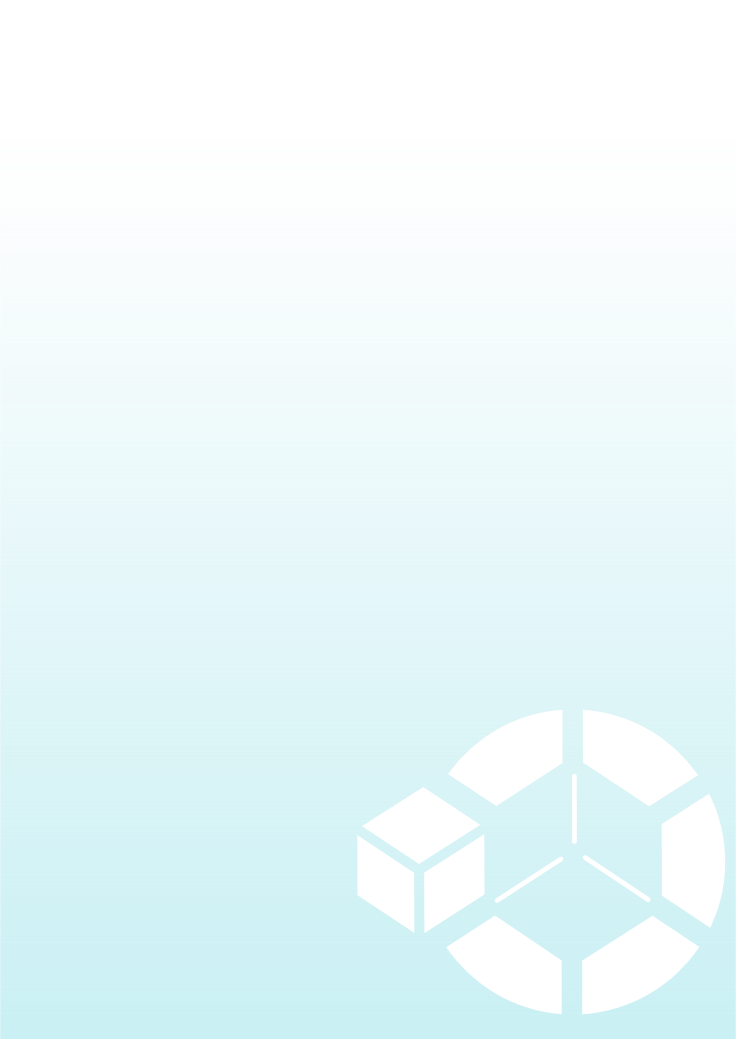
\includegraphics[width=\paperwidth,height=\paperheight]{Bilder/Bild1.png}};

% Inlcude TUHH-Logo and IEET-Logo
\begin{minipage}{.5\textwidth}
\ifthenelse{\equal{\Sprache}{0}}{

\includegraphics[height=50pt]{Bilder/TUHH_logo-wortmarke_de_rgb.png}
}{
\includegraphics[height=50pt]{Bilder/TUHH_logo-wortmarke_de_rgb.png}}
\end{minipage}% This must go next to `\end{minipage}`
\begin{minipage}{.5\textwidth}
\begin{flushright}
\ifthenelse{\equal{\Sprache}{0}}{
\includegraphics[height=45pt]{Bilder/office_rgb_ieet_de.png}}{
\includegraphics[height=50pt]{Bilder/office_rgb_ieet_en.png}}
\end{flushright}
\end{minipage}

% Titel der Arbeit
%\hspace{1cm}\\ % muss hier stehen ansonsten wird der vspace nicht akzeptiert
\begin{center}
		\vspace{5cm}
		{\ifthenelse{\equal{\Sprache}{0}}{\DeutscherTitelDerArbeit}{\EnglischerTitelDerArbeit}
		\Large{\textbf{}}}
	\end{center}
	\begin{center}
		{\textbf{\VornameDesStudenten \ \NachnameDesStudenten}}
\end{center}

\end{titlepage}
\clearpage
\thispagestyle{empty}
\cleardoublepage

%| Titelseite
\thispagestyle{plain}                          % keinen Header für Deckblatt
% !TeX root =../main.tex

\begin{titlepage}
%\thispagestyle{empty}
\setlength{\voffset}{-1cm}
\setlength{\footskip}{0pt}

\vspace*{16cm}

\begin{flushright}
\VornameDesStudenten \ \NachnameDesStudenten \\[0.3cm]
\Matrikelnummer \\[0.3cm]
\Studiengang \\ [0.3cm]
\ArtDerArbeit \\[0.3cm]
\IEETNumber \\[0.3cm]
\Abgabe \\[0.3cm]
\ifthenelse{\equal{\Sprache}{0}} % Ändert die Bezeichnungen auf gemäß der Sprache auf Prüfer/Examiner bzw. Betreuer/Supervisor.
				{
Prüfer: Prof. Dr.-Ing. Christian Becker \\[0.3cm]
\ifthenelse{\equal{\MScBSc}{2}}{Zweitprüfer: \Zweitpruefer \\[0.3cm]}{}
Betreuer: \BetreuerE \ifthenelse{\equal{\BetreuerZ}{Betreuer 2}}{}{\text{,\BetreuerZ}} \\[0.3cm]}
{
Examiner: Prof. Dr.-Ing. Christian Becker \\[0.3cm]
\ifthenelse{\equal{\MScBSc}{2}}{Zweitprüfer: \Zweitpruefer \\[0.3cm]}{}
Supervisor: \BetreuerE \ifthenelse{\equal{\BetreuerZ}{Betreuer 2}}{}{\text{, \BetreuerZ}}
}
\end{flushright}
\end{titlepage}
\newpage
\thispagestyle{empty} 
\cleardoublepage

%| Fußnoten
\setlength{\parindent}{0pt}                    % Verhindert Einrückes des Textes nach Absätzen, Abb./ Tab./ Formeln
\setlength{\footnotesep}{9pt}                  % Legt den Abstand zwischen zwei Fußnotentexten am unteren Seitenrand fest


%| Kopfzeile
\pagestyle{scrheadings}                        % Eigene Kopfzeile
  %\clearscrheadfoot                            % Löscht bisherige Kopfzeilen
  \clearpairofpagestyles
  \automark[section]{chapter}                  % Automatischen makieren [Rechte Seite]{Linke Seite}
  \ihead[]{\leftmark}                          % inner(oben) = linke Seite
  \ohead[]{\rightmark}                         % outer(oben) = rechte Seite
  \ohead[\pagemark]{\pagemark}                 % outer(oben) = die Seitenzahl immer außen
  \KOMAoptions{headsepline=true, headsepline=0.4pt}  % Erstellt eine Linie in Kopfzeile unter der Seitennummer etc.


%| Zeilenabstand
\doublespacing                             	   % 2-facher Zeilenabstand


\thispagestyle{empty}                  
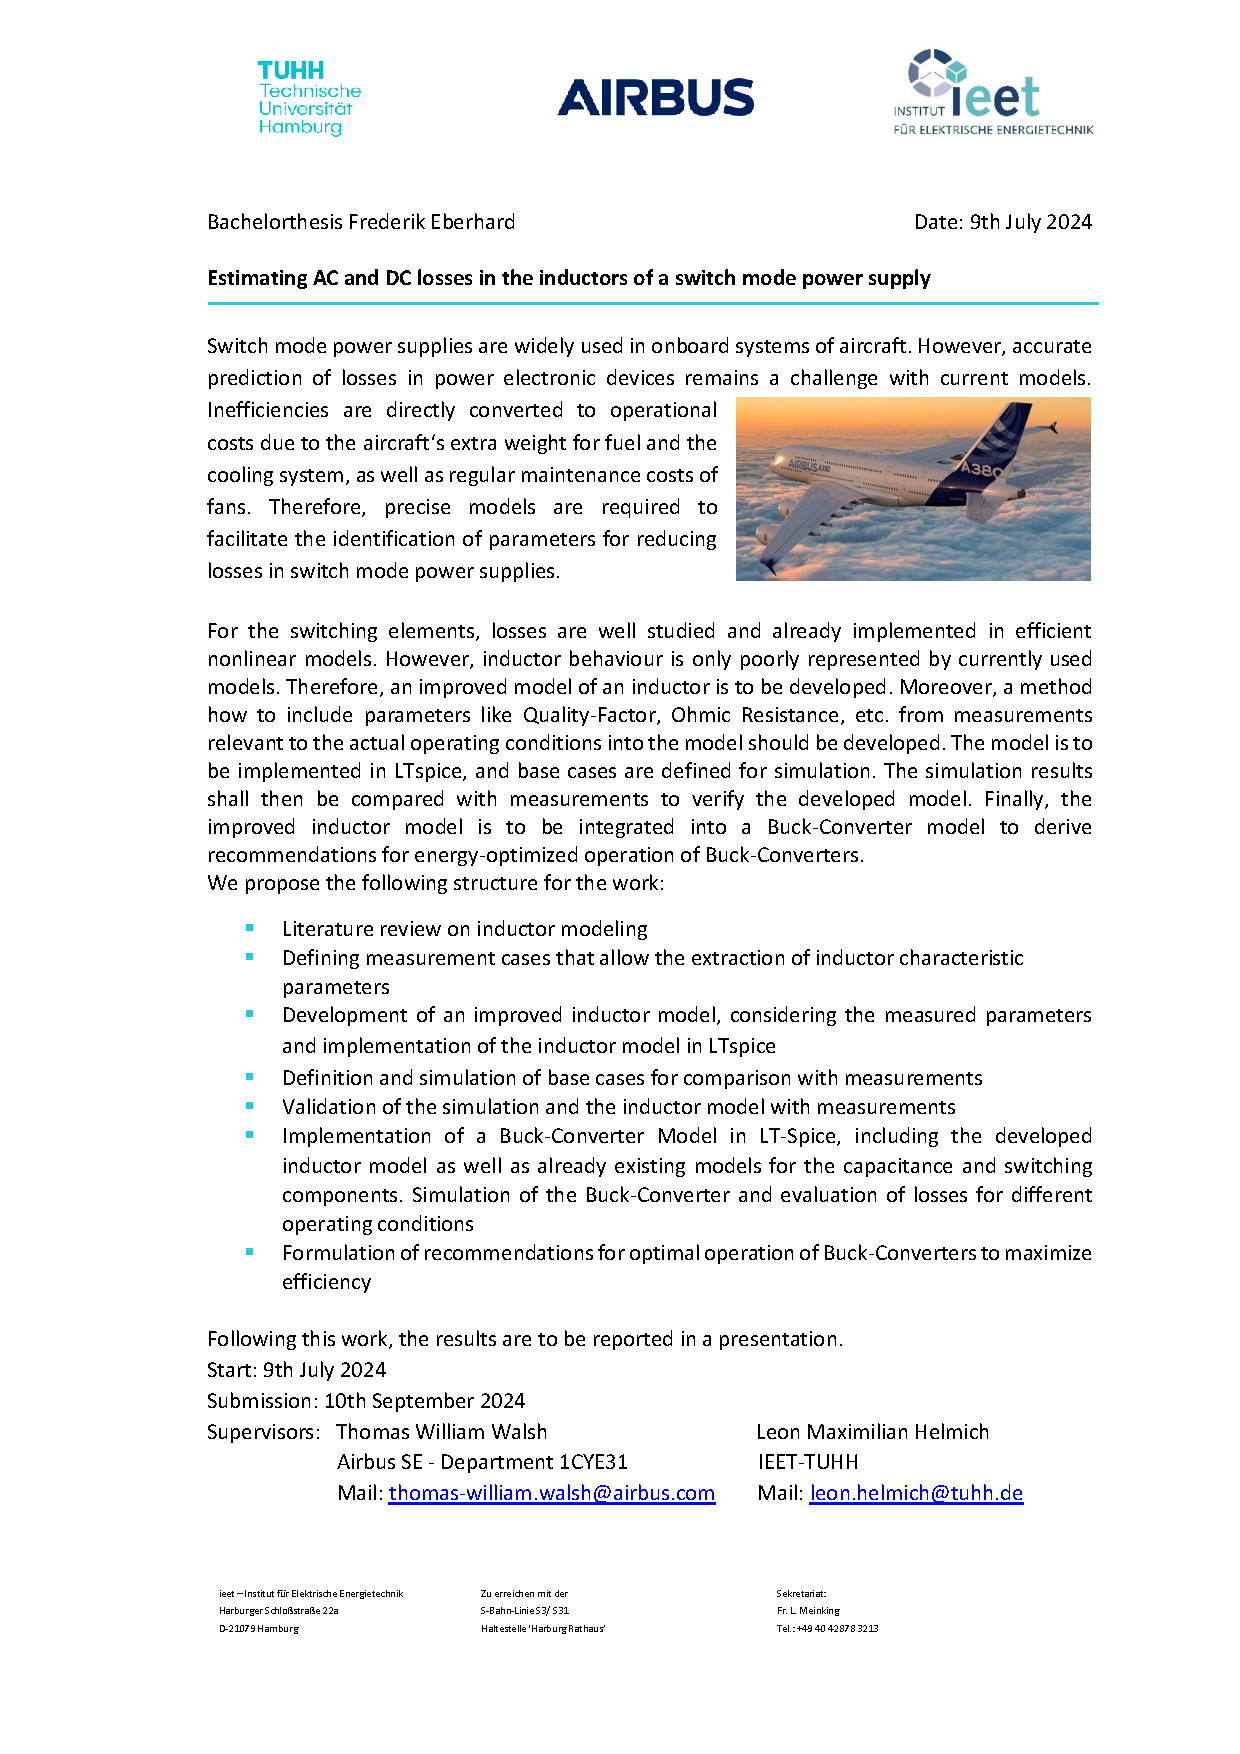
\includepdf[offset= -25 -15]{Kapitel/Aufgabenstellung.pdf}		% eventuell sind hier die Offsets anders zu setzen.

\newpage
\thispagestyle{empty}
\cleardoublepage 

%| ~ Anmk: Ab hier werden Seitenzahlen gezählt
\pagenumbering{roman}                                 						% Römische Seitenzahlen bis Beginn des Inhalts

%/Kurzfassung
% !TeX root =../main.tex

\chapter*{Kurzfassung}   \label{cha:Kurzfassung}

Wie bereits in der Schule gelernt, besitzen unterschiedliche Arten von Texten unterschiedliche förmliche Kriterien. Eine besondere Art eines Textes ist die wissenschaftliche Abschlussarbeit im Rahmen eines Studiums. Die Anforderungen an eine solche Arbeit ist in den unterschiedlichen Fachgebieten, wie z.B. Mechanik, Elektrotechnik, oder Verfahrenstechnik, zum Teil unterschiedlich, da sich historisch andere Konventionen ergeben haben. Aus diesem Grund soll Ihnen diese Vorlage für Ihre Abschlussarbeit dienen und gleichzeitig ein Art Wegweiser für die förmlichen sowie inhaltlichen Anforderungen bieten, die das Institut für elektrische Energietechnik an eine Abschlussarbeit stellt.

Dabei orientiert sich diese Vorlage an dem geforderten Aufbau einer Abschlussarbeit. Zu jedem Unterpunkt werden kurze Beispiele bzw. eine kurze Beschreibung zu den inhaltlichen Erwartungen gegeben. Besonders hervorzuheben ist dabei das Kapitel \ref{sec:fundamentals}, in dem eine Vielzahl an Beispielen und Latex Implementierungen ausgeführt wird. Außerdem ist in Kapitel \ref{sec:ausblick} eine Zusammenfassung für den Aufbau und den Inhalt der Arbeit zu finden. 

Sämtliche Texte in dieser Vorlage müssen durch Ihren Text, Überschriften, Abkürzungen usw. ersetzt werden. Ebenso müssen die Einstellungen in der Datei \enquote{Einstellung.tex} angepasst werden. 


\setlength{\headheight}{22.00473pt}
\setlength{\footheight}{22.00473pt}
\newpage
\thispagestyle{empty} 
\cleardoublepage


%/Abstract
% !TeX root =../main.tex

\chapter*{Abstract}   \label{cha:Abstract}
Due to the high amount of consumer electronic devices being used nowadays, \ac{SMPS} play a critical role in the electrical infrastructure. As millions of them are constantly used, drawing power from the electrical grid, even small amounts of power losses have a big impact on the overall energy expended. Because of this, maximising the efficiency of newly produced power supplies is crucial. However, the efficiency of a given \ac{SMPS} is affected by many different factors, complicating this task. Simulation, therefore, is a crucial step in the design process of \acp{SMPS}. With it, the vast amount of possible components, designs and settings can be reduced to a handful of optimal combinations suited for a specific application purpose. Currently, however, the models used for simulations of inductors, which are the key component in \ac{SMPS}, are not able to represent their losses well enough.\\
This thesis presents a novel approach to simulate the inductor of a \ac{SMPS} in LTspice, taking into account different sources of losses. Focusing on three different approaches to recreate the behaviour of multiple inductors, the non-linearities of these inductors are explained and implemented in LTspice. A buck converter is used to present the workings of \acp{SMPS}. Making use of provided switching element models, the created inductor models are inserted into the simulation of the buck converter. The same buck converter is then also recreated physically, enabling the direct comparison of the simulated and measured inductor behaviour. Operated at different switching frequencies, the losses of the inductor and the switching elements are compared. The results of the simulation are then shown to help in the prediction of the optimal switching frequency range for each buck converter, maximising efficiency.

\newpage
\thispagestyle{empty} 
\cleardoublepage

% ---- optional ---- 
%/Danksagung
\ifthenelse{\equal{\MitDanksagung}{1}}{
% !TeX root =../main.tex

\chapter*{\ifthenelse{\equal{\Sprache}{0}}{Danksagung}{Acknowledgement}} \label{Danksagung}

Diese Seite ist optional.\\[2cm]

\Ort , \printdayoff \today \printdayon
\newpage
\thispagestyle{empty} 
\cleardoublepage}{}


%|============================================================================|
%| Verzeichnisse                                                              |
%|============================================================================|

%| Inhaltsverzechnis
\tableofcontents       % Erstellt automatisch ein Inhaltsverzeichnis

\newpage
\thispagestyle{empty}
\cleardoublepage
\pagestyle{plain}
%/ Abkürzungsverzeichnis
\chapter*{List of Abbreviations}                       
% !TeX root =../main.tex

\begin{acronym}[IWESsss] % IWESssss: gibt den Abstand beim Druck zwischen den Abkürzungen und den Langformen an
        \acro{ECM}[ECM]{equivalent circuit model}
        \acrodefplural{ECM}[ECM]{equivalent circuit models}
        \acro{HS}[HS]{high side}
        \acro{LS}[LS]{low side}
        \acro{CCM}[CCM]{continuous current mode}
        \acro{DC}[DC]{direct current}
        \acro{AC}[AC]{alternating current}
        \acro{MOSFET}[MOSFET]{metal oxide silicon field effect transistor}
        \acrodefplural{MOSFET}[MOSFETs]{metal oxide silicon field effect transistors}
        \acro{GaNFET}[GaNFET]{gallium nitride field effect transistor}
        \acrodefplural{GaNFET}[GaNFETs]{gallium nitride field effect transistors}
        \acro{SMPS}[SMPS]{switch mode power supply}
        \acrodefplural{SMPS}[SMPS]{switch mode power supplies}
        \acro{ZVS}[ZVS]{zero voltage switching}
        \acro{ZCS}[ZCS]{zero current switching}
        \acro{RMS}[RMS]{root mean square}
\end{acronym}
\thispagestyle{empty}

\newpage
\thispagestyle{empty}
\cleardoublepage 

%/Formelzeichen
\section*{List of Symbols}             
% !TeX root =../main.tex

\begin{xltabular}{\textwidth}{>{$} m{3cm}<{$} m{12cm}}
	a_t & Aktion zum Zeitpunkt $t$\\
	a_{t+1} & Aktion zum Zeitpunkt $t+1$\\
	\mathcal{D} & Puffergröße\\
	e_t & Sammlung von vorherigen Zuständen aus dem Pufferspeicher\\
	I & Stromstärke\\
	P_{\mathrm{G}} & Antriebsleistung der Turbine bzw. Erzeugerleistung (in MW)\\
	Q^* & Maximaler Q-Wert aus aktuellem Zustand und Aktion\\
	Q_\theta & Primärnetz\\
	Q_\theta' & Zielnetz\\
	R & Elektrischer Widerstand\\
	\mathrm{R(s_t,a_t)} & Belohnungsfunktion\\
	r_t & Belohnung zum Zeitpunkt $t$\\
	s_t & Zustand zum Zeitpunkt $t$\\
	s_{t+1} & Zustand zum Zeitpunkt $t+1$\\
	T & Boltzmann Temperaturparameter\\
	U & Spannung\\
		\\
	\alpha_\mathrm{r} & Lernrate\\
    \gamma & Diskontinuierungsfaktor\\
    \epsilon & Explorationsparameter\\
	\theta & Gewichtsparameter des Primärnetzes\\
	\theta' & Gewichtsparameter des Zielnetzes\\
	\pi(s_t,a_t) & Strategie des RL-Algorithmus\\
	\tau & Aktualisierungsrate des Zielnetzwerks\\
	\\
	\mathrm{H_2O} & Wasser\\
	\mathrm{OH^-} & Hydroxidion\\
	\mathrm{O_2} & Sauerstoff\\
\end{xltabular}
\newpage
\thispagestyle{empty}
\cleardoublepage 

%| Kopfzeile
\pagestyle{scrheadings}                        % Eigene Kopfzeile
\clearpairofpagestyles                            % Löscht bisherige Kopfzeilen
\automark[section]{chapter}                  % Automatischen makieren [Rechte Seite]{Linke Seite}
\ihead[]{\leftmark}                          % inner(oben) = linke Seite
\ohead[]{\rightmark}                         % outer(oben) = rechte Seite
\ohead[\pagemark]{\pagemark}                 % outer(oben) = die Seitenzahl immer außen
\KOMAoptions{headsepline=true,       % Syntax error corrected 8.2.2020
            headsepline=0.4pt}
%\setheadsepline{.4pt}                        % Erstellt eine Linie in Kopfzeile unter der Seitennummer etc.

%|============================================================================|
%| Einbinden der Kapitel                                                      |
%|============================================================================|

\pagenumbering{arabic}	% Vorher römische Seitenzahlen, ab hier arabische. Fängt automatisch wieder bei 1 an

%/Einleitung
% !TeX root =../main.tex

\chapter{Einleitung} 
\label{sec:intro}
\todo[inline]{Introduction: What are SMPS, what are GaNFETs?, Why study loss in inductors}


Es geht zunächst um die Gliederung der Abschlussarbeit und dann um die Anforderungen an das erste Kapitel, die Einleitung. 

\section{Gliederung einer wissenschaftlichen Arbeit}
Im Allgemeinen können Abschlussarbeiten, egal ob Studien-, Bachelor- oder Masterarbeiten in gleicherweise strukturiert und gegliedert werden. Dieser allgemeine Aufbau wird im Folgenden beschrieben. In Einzelfällen, d.h. bei speziellen Themen können auch leichte Anpassungen nötig sein.\par

Formal gesehen hat jede wissenschaftliche Arbeit folgende Bestandteile, die Sie auch als generisches Inhaltsverzeichnis verstehen können:
\begin{itemize}
    \item[] 0a. Kurzzusammenfassung (Abstract)
	\item[] 0b. Abkürzungen
	\item[] 0c. Formelzeichen
    \begin{enumerate}
	    \item Einleitung
	    \item Grundlagen
	    \item Lösungs-/Modellierungs-/Implementierungsteil/Versuchsaufbau
	    \item Anwendungsbeispiele, -szenarien, Messungen und Diskussion der Ergebnisse
	    \item Zusammenfassung und (optionaler) Ausblick
	    \item Literaturverzeichnis
	\end{enumerate}
\item[] Anhang/Anhänge
\end{itemize}

Grundlagenteil und Implementierungsteil können dabei, je nach Erfordernis, jeweils aus einem oder mehreren Kapiteln bestehen. Diese beiden Teile machen zusammen etwa zwei Drittel des Gesamtumfangs aus. Die Einleitung führt zur eigentlichen Arbeit hin. Sie wirkt, bildlich gesprochen, wie ein Trichter: alle für die Arbeit relevanten Problembereiche werden hineingesteckt, heraus kommt die fokussierte Themenstellung Ihrer Arbeit. Die Arbeit nimmt in ihrem Detaillierungsgrad zu. Lediglich in Zusammenfassung und Ausblick weitet sie sich wieder ins Allgemeine. Vorwärtsverweise sollten Sie möglichst vermeiden. Wenn Sie meinen, solche zu benötigen, untersuchen Sie, ob Sie sie nicht durch Umstellung umgehen können. Rückwärtsverweise sollten dagegen auftreten. Sie verankern den Grundlagenteil mit der Einleitung, die Implementierung mit den Grundlagen, Beispiele mit Grundlagen und Implementierung. Die Arbeit sollte auch einen geschlossenen Eindruck auf einer bestimmten Abstraktionsebene bieten, ohne dass ein Leser gezwungen ist, die gesamte Arbeit zu lesen. Es sollte daher möglich sein, nur die Einleitung, eventuell zusammen mit Zusammenfassung und Ausblick, zu lesen, um sich einen Überblick über die Ergebnisse der Arbeit zu verschaffen. Jemand, der sich nicht für die Implementierung interessiert, sollte mit Einleitung und Grundlagenteil einen detaillierten Einblick in die verwendeten Grundlagen und entwickelten Modelle Ihrer Arbeit gewinnen können, das Für und Wider der verschiedenen Entwurfsalternativen sehen sowie die Begründung für den ausgewählten Ansatz finden. Achten Sie darauf, dass im Implementierungsteil keine neuen Grundlagen vorgestellt oder gar neue Begriffe eingeführt werden. In einem solchen Fall deutet alles darauf hin, dass der Grundlagenteil unvollständig ist. Wer sich schließlich für die Güte der Implementierung interessiert oder Detailabläufe anhand beispielhafter Szenarien verstehen will, muss sicherlich die ganze Arbeit lesen.
Im Folgenden sollen die einzelnen Abschnitte etwas detaillierter betrachtet werden. Dabei wird von einer "idealen" wissenschaftlichen Arbeit ausgegangen. "Ideal" bezieht sich dabei nicht nur auf Ihre Leistung, sondern auch auf das gestellte Thema, das entsprechend den dargelegten Punkten auch etwas hergeben muss. Versuchen Sie nicht, künstlich an Stellen etwas zu erzeugen, wo nichts zu holen ist.\newline

\textit{0a. Kurzzusammenfassung}\par
Die Kurzzusammenfassung ist vergleichbar mit Klappentexten bei wissenschaftlichen Büchern. Sie soll in wenigen Sätzen die Arbeit zusammenfassen und das Interesse des Lesers wecken, die ganze Arbeit zu lesen. 
Die Kurzzusammenfassung soll von einem auf diesem Feld interessierten Forscher gelesen und verstanden werden können. Der Text soll dem Leser die Information geben, welches Problem mit welchen Lösungsansätzen behandelt wurde. Anschließend sollen die Kern-Ergebnisse der Arbeit in wenigen Sätzen zusammengefasst werden.

Beachten Sie hierbei, dass die Problemstellung nicht ausführlich erklärt werden muss, sondern nur genannt wird. Gleiches gilt für die Lösungsansätze. Schlankheit und Präzision sind in diesem Abschnitt von zentraler Bedeutung. Zusätzlich ist ein „Abstract“, also die englische Version der Kurzzusammenfassung, je nach Länge auf einer separaten Seite oder auf derselben Seite wie die Kurzzusammenfassung zu erstellen (siehe Vorlage).\newline

\textit{0b. Abkürzungen}\par
Bei besonders langen Ausdrücken, die wiederholt genannt werden oder Ausdrücken mit bekannten Kurzformen, ist es möglich, Abkürzungen zu verwenden. Diese Abkürzungen sind in \verb|abkuerzung.tex| zu hinterlegen und entsprechend in den Text mit \verb|\ac{}| einzufügen. Durch diese Form der Referenzierung wird sichergestellt, dass der Ausdruck bei der ersten ein Erwähnung wie folgt dargestellt wird: \ac{WKA}. Jedoch bei jeder weiteren Erwähnung nur noch so: \ac{WKA} bzw. im Plural \acp{WKA}.  
Abkürzungen sollten den Lesefluss nicht stören, sondern unterstützen. Gehen Sie daher sparsam mit Abkürzungen um.
\newline



\textit{0c. Formelzeichen}\par
Bei der Verwendung von Formeln, sollten alle verwendeten Parameter und Indizes an dieser Stelle übersichtlich protokolliert werden.





\section{Was steht in der Einleitung?}
\label{sec: WsidE}
Ziel der Einleitung ist es, zum eigentlichen Thema der Arbeit hinzuführen sowie dem Leser einen inhaltlichen Überblick über die Arbeit zu geben. Die Einleitung muss von jedem Elektrotechniker verstanden werden können. Abstraktionsniveau, Sprache usw. sind also entsprechend zu wählen.
Fangen Sie aber nicht bei zu grundlegend Dingen an. Als Anhaltspunkt können Sie alles voraussetzen, was in den Pflichtveranstaltungen Ihres Studiums behandelt wurde. Die über den Satz an "Grundbegriffen" hinausgehende Fachsprache muss eingeführt werden. Die verschiedenen "Quellbereiche" für Probleme und Lösungsansätze können in verschiedenen Abschnitten (Unterkapiteln) dargelegt werden. Sie spannen mit der Einleitung den Raum auf, in dem Sie sich im Grundlagenteil Ihrer Arbeit bewegen. Hieraus muss die fokussierte Problemstellung Ihrer Arbeit erwachsen. Belegen Sie, wenn möglich, dass Sie ein wichtiges Problem angehen (neuer Algorithmus, wirtschaftlichere Lösung, Qualität der Lösung, Verbesserung der Umweltverträglichkeit einer Lösung). Geben Sie die Highlights Ihrer Arbeit an. Die Einleitung muss für den Leser die Frage beantworten, ob sich für ihn das Lesen weiterer Kapitel oder der gesamten Arbeit lohnen könnte. Im Überblick über den Rest der Arbeit sollten die prinzipielle Vorgehensweise, die Highlights usw. sichtbar werden. Sie geben dem Leser damit eine Orientierung, wo er die ihn eventuell interessierenden Dinge findet. Üblich ist, dabei kapitelweise vorzugehen. Der "rote Faden" Ihrer Arbeit sollte dann jedem Leser offensichtlich werden.
Zusammenfassend ist es folglich ratsam, die Einleitung in drei Sinnabschnitte zu unterteilen:
\begin{itemize}
    \item{\textbf{Einführung in die Problematik } $\boldsymbol{\rightarrow{}}$   Hier wird herausgearbeitet, warum die Themenstellung es wert ist, sie zu untersuchen und gleichzeitig eine Einbettung in den energietechnischen Kontext vollzogen.}
    \item{ \textbf{Aktueller Stand der Literatur } $\boldsymbol{\rightarrow{}}$  Hier wird herausgearbeitet, was der aktuelle Stand der Literatur auf dem Themengebiet ist (inkl. Nennung von Quellen) und deutlich aufgezeigt, wie sich die vorliegende Arbeit davon abgrenzt und was der Mehrwert („neu“) an der eigenen Arbeit ist.}
    \item{\textbf{Ziel und Aufbau der Arbeit} $\boldsymbol{\rightarrow{}}$  Hier wird das Ziel der Arbeit klar formuliert und im weiteren der Aufbau der Arbeit (kapitelweise) beschrieben. Dem Leser soll hierdurch der Zusammenhang zwischen den Kapiteln sowie zusätzlich auch der rote Faden deutlich werden (und zusätzlich auch der rote Faden)}
\end{itemize}

\SI{}{\ohm}



	% einfügen von inhalt/inhalt.tex
\newpage
\thispagestyle{empty} 
\cleardoublepage

%/Kapitel2
% !TeX root =../main.tex

\chapter{Fundamentals} \label{sec:fundamentals}
In this chapter, first the workings of a buck converter are discussed in section \ref{sec:the_buck_converter}. After that, the different types of losses occurring in a buck converter are explained in sections \ref{sec:losses_in_switching_elements} and \ref{sec:losses_in_the_inductor}, first focusing on the losses occurring in the switching elements and then explaining the losses occurring in the inductor. 
\section{The buck converter}
\label{sec:the_buck_converter}
DC to DC converters come in many different topologies, one of which is the synchronous buck converter seen in figure \ref{fig:synch_buck_converter_2}. Buck converters are step down converters, taking in a high voltage and outputting a low voltage. In contrast to other methods of voltage reduction, converters aim to have close to zero power loss across them. This results in the current at the output being greater than the current at the input. \\
\begin{figure}[H]
    \centering
    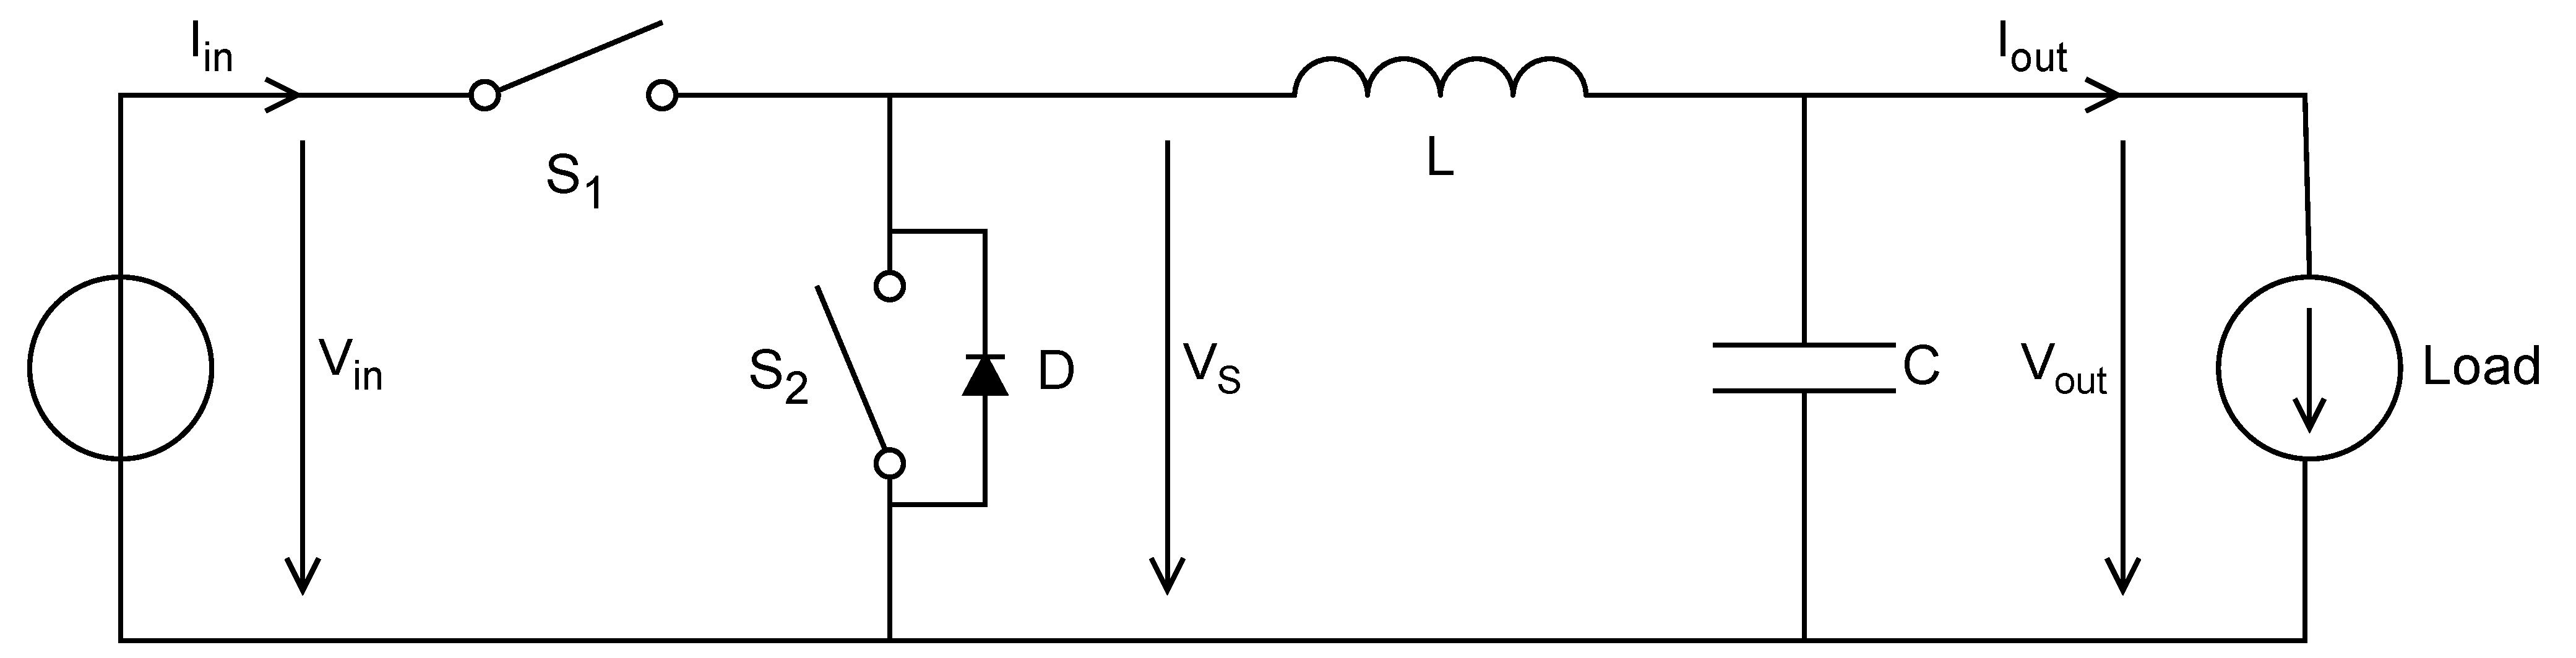
\includegraphics[width=1\linewidth]{Bilder//Kapitel2/SBC_2_D.pdf}
    \caption{Synchronous Buck Converter}
    \label{fig:synch_buck_converter_2}
\end{figure}
As shown in figure \ref{fig:stages_of_a_buck_converter.}, to function buck converters repeatedly charge and discharge the inductor $L$ by switching the two switches with a given frequency and duty cycle. Closing switch $S_1$, also refereed to the \ac{HS} switch, allows current to flow from the source to the load through the inductor. The inductor resists the change in current, charging its magnetic field while increasing the current linearly. After a certain time $t_1$, switch $S_1$ is opened, stopping the current flowing in from the source. The current through the inductor however is forced to continue flowing, now discharging the inductor through the diode D connected to the switch $S_2$, the \ac{LS} switch. To avoid short circuits, $S_2$ is not closed simultaneously with the opening of $S_1$ but is instead delayed by a dead time $t_{d}$. During dead time the negative voltage drop $V_d$ across the diode can be observed, After this dead time, switch $S_2$ is closed, and the inductor discharges for the rest of the period $T_1$. Switch $S_2$ opens again and after a second short dead time, $S_1$ connects the circuit back to the power source. The naming-convention of the dead times follows the signal supplied to the \ac{HS} switch. Opening the switch is done by the falling edge of the signal, resulting in the dead time to be named the falling edge dead time $t_{df}$. Similarly, on the rising edge of the signal to $S_1$ the dead time is called the rising edge dead time $t_{dr}$.

\begin{figure}[H]
    \centering
    \includegraphics[width=1\linewidth]{Bilder//Kapitel2/BuckConverter_Stages_1_1.pdf}
    \caption{Internal operation of a buck converter}
    \label{fig:stages_of_a_buck_converter}
\end{figure}

As long as the magnetic field of the inductor is not fully discharged by the time the \ac{HS} is closed again, the buck converter operates in \ac{CCM}. In \ac{CCM} the current through the inductor can be viewed as the superposition of two functions. First, a \ac{DC} that flows through the load labelled $I_{out}$ and secondly a triangle shaped \ac{AC}, called the ripple current $I_{L_r}$. Depending on the switching frequency, duty cycle and inductance, this ripple current can be more or less pronounced. The output capacitor is used to stabilise the current at the output gate, stopping the ripple current from reaching the load. It therefore acts as an ideal low pass filter, keeping both output current and voltage constant.\\
In real synchronous buck converters, there is no separate diode connected across the \ac{LS} switching element. Instead, both commonly used \acp{MOSFET} and \acp{GaNFET} are able to conduct reverse current, acting similarly to a diode. \\

To calculate the dependency between the output and input voltages, the current across the inductor is analysed. For any type of inductor, the relationship between inductor current and inductor voltage is given by \ref{eq:inductor_current}.
\begin{equation}\label{eq:inductor_current}
    i_L(t) = \frac{1}{L} \cdot \int_{0}^{t} v_L(\tau) \,d\tau
\end{equation}
As for constant currents, the voltage experienced by an inductor is zero, only the change in current affects the inductor voltage and therefore in turn the output voltage. The time for which a specific voltage is applied to the inductor is given by the on-time and off-time of the switch. These are characterised by the time it takes to complete an entire switching cycle $T_s$ and the fraction of that time they each take up, denoted by the duty cycle $D$.\\
For the on-time of the switch, the change in current $\Delta i_{L_{on}}$ is given by equation \ref{eq:inductor_current_on}, as the inductor's voltage is equal to the difference in voltage between the input and output gate. During the off-time, the inductors current falls as the input is no longer connected. Excluding dead time, as $T_s >> (t_{df} + t_{dr})$ the voltage across the inductor is equal to the output voltage $V_{out}$. This results in equation \ref{eq:inductor_current_off} describing the off-time current change. 
\begin{align}
    \Delta i_{L_{on}} &= \frac{1}{L} \cdot (V_{in} - V_{out}) \cdot D \cdot T_{s}       \label{eq:inductor_current_on}\\
    \Delta i_{L_{off}} &\approx \frac{1}{L} \cdot V_{out} \cdot (1-D) \cdot T_{s}     \label{eq:inductor_current_off}\\
\end{align}
For steady-state operation, the changes in the inductor current have to cancel each other out, as the current at the beginning of the cycle has to match the current at the end of it. Using this relation, given in equation \ref{eq:inductor_current_cancel}, results in equation \ref{eq:duty_cycle}. Neglecting the dead time causes the output voltage only to depend on the input voltage and the duty cycle. 
\begin{align}
    \Delta I_{L_{on}} &+ \Delta I_{L_{off}} = 0                                         \label{eq:inductor_current_cancel}\\
    D &\approx \frac{V_{out}}{V_{in}} 
        \label{eq:duty_cycle}
\end{align}


\section{Buck converter losses}\label{sec:losses_in_bc}
The synchronous buck converter's three main components, the capacitor, switching elements and inductor all contribute to power loss and are to a certain degree frequency-dependent. The capacitive losses are not discussed in great detail in this thesis, as they are usually responsible for less than 1\% of the total losses \cite{An_Accurate_Approach_for_Calculating_the_Efficiency_of_a_SBC}.
\subsection{Losses in the switching elements}\label{sec:losses_in_switching_elements}
The main causes of losses in switching elements are conductive losses, dead time losses and switching losses. Gate drive losses and capacitive losses are not explored in this thesis, as they are minimal compared with the before-mentioned causes. \\
A sixth type of loss, the reverse recovery loss resulting from the body diode of \acp{MOSFET}, does not play a role in this thesis, as it focuses exclusively on \acp{GaNFET}, which lack a body diode. This, however, does not exempt \acp{GaNFET} from conducting a current in reverse. Applying a negative drain-source voltage $V_{DS}$ results in diode-like behaviour, inducing a negative drain-source current $I_{DS}$. To model this, a diode is incorporated into the \ac{ECM} as shown in figure \ref{fig:GaNFET_ECM} \cite{Does_GaN_Have_a_Body_Diode}.
\begin{figure}[H]
    \centering
    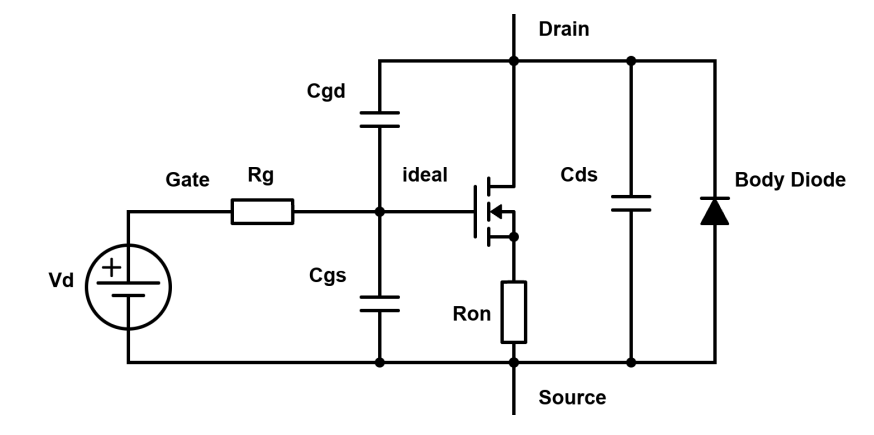
\includegraphics[width=0.75\linewidth]{Bilder//Kapitel2/GaNFET_ECM.png}
    \caption{Equivalent Circuit Model of a GaNFET}
    \label{fig:GaNFET_ECM}
\end{figure}
\subsubsection{Conductive Losses}
The conductive losses arise directly by the resistive impedance of the \ac{GaNFET} $R_{DS_{on}}$ during on-time. The current flowing through the \ac{HS} \ac{GaNFET} is equal to the current through the inductor during the charging phase $t_1$ and has the shape of a raised saw tooth wave. Calculating the \ac{RMS} value of the current necessary for the power calculation can be done with the equation \ref{eq:rms_raised_saw_tooth}. 
\begin{equation}
    I_{rms} = \sqrt{\frac{t_{on}}{T_s} \cdot \left( I_{min}\cdot I_{max}+\frac{\left(I_{max}-I_{min}\right)^2}{3}\right)} \label{eq:rms_raised_saw_tooth}
\end{equation}
The minimum and maximum currents through the \ac{GaNFET}, are equal to the minimum and maximum inductor currents $(I_{out}-\frac{\Delta I_{L_r}}{2})$ and $(I_{out}+\frac{\Delta I_{L_r}}{2})$. Their difference is directly expressed by the amplitude of the ripple current $\Delta I_{L_r}$. Inserting this and accounting for the duty cycle results in equation \ref{eq:rms_HS_GAN_1}. This simplifies to equation \ref{eq:rms_HS_GAN_2}. 
\begin{align}
    I_{rms_{HS}} &= \sqrt{\frac{T_s\cdot D}{T_s} \cdot \left(\left(I_{out}-\frac{\Delta I_{L_r}}{2}\right)\cdot \left(I_{out}+\frac{\Delta I_{L_r}}{2}\right)+\frac{\left(I_{L_r}\right)^2}{3}\right)}\label{eq:rms_HS_GAN_1}\\
    &=\sqrt{D \cdot \left(I_{out}^2 - \frac{\Delta I_{L_r}^2}{12}\right)}\label{eq:rms_HS_GAN_2}
\end{align}
Since the power loss over a resistor is equal to the resistors value times the square of the current, the resulting conduction power loss for the \ac{HS} \ac{GaNFET} is expressed by equation \ref{eq:Pon_HS_GAN}. As the \ac{LS} \ac{GaNFET} experiences the falling edge of the inductors current, the minimum and maximum currents are identical to the \ac{HS}. The \ac{LS} conduction losses thereby follow the same form, only differing in the on-time fraction being $\left(1-D\right)$.
\begin{align}
    P_{con,HS} &= R_{ds_{on}} \cdot D \cdot \left(I_{out}^2 - \frac{\Delta I_{L_r}^2}{12}\right)\label{eq:Pon_HS_GAN}\\
    P_{con,LS} &= R_{ds_{on}} \cdot \left(1-D\right) \cdot \left(I_{out}^2 - \frac{\Delta I_{L_r}^2}{12}\right)\label{eq:Pon_LS_GAN}
\end{align}
Conduction losses are therefore only indirectly dependent on frequency, as the amplitude of the ripple current is frequency-dependent. However, in normal operation $I_{out}^2 >> \frac{\Delta I_{L_r}^2}{12}$, allowing the \ac{RMS} current to be approximated by the product of duty cycle and output current, removing the frequency dependence. 
\subsubsection{Dead Time Losses}
During both dead times, a current is conducted by the \ac{LS} \ac{GaNFET} via its "body diode", as it has a higher potential at its source than at its drain. As long as $t_{df}, t_{dr} << T_s$ the current during the dead time can be approximated to be constant. For the falling edge dead time $t_{df}$ this results in the maximum inductor current $(I_{out}+\frac{\Delta I_{L_r}}{2})$ flowing through the "body diode". The energy lost during this dead time is the momentary power loss given as the product of this current and the voltage across the diode $V_D$ times the duration of the dead time $t_{df}$ and is given by equation \ref{eq:dead_time_energy}. 
\begin{equation}\label{eq:dead_time_energy}
    E_{t_{df}} = V_D \cdot (I_out + \Delta I_{L_r}^2) \cdot t_{df}
\end{equation}
As this energy is lost every switching cycle, the over all falling edge dead time power loss is the energy multiplied by the switching frequency $f_s$. The same approach is used for the rising edge dead time $t_{dr}$. Here the current is the minimum inductor current $(I_{out}-\frac{\Delta I_{L_r}}{2})$ and the duration changes to $t_{dr}$. Summing up both dead time losses and factoring out the voltage and switching frequency, as they stay constant for both cases, the total dead time power loss is given by equation \ref{eq:dead_time_power_loss}.
\begin{equation}\label{eq:dead_time_power_loss}
P_{td} = V_D \cdot f_s \cdot \left(t_{df} \cdot \left(I_{out} + \Delta I_{L_{pp}}^2\right) + t_{dr} \cdot \left(I_{out} - \Delta I_{L_{pp}}^2\right)\right)    
\end{equation}
The source-drain $V_{sd}$ for \acp{GaNFET} is usually higher than the body diode voltage drop in \acp{MOSFET}, increasing the importance of minimizing dead time in \ac{GaNFET} \ac{SMPS}. \\

\subsubsection{Switching Losses}

Switching losses are differentiated between \textit{hard switching}, where the power losses are high, and \textit{soft switching}, where the power losses are close to zero. \textit{Hard switching} is analysed first to explain how switching losses occur and how \textit{soft switching} can minimize the losses.\\
In \acp{GaNFET}, during the transition between non-conducting and conducting, both a high current flows through it and a high voltage drop occurs. This results in power loss in the switch. To simplify the calculations, we assume the voltages and currents rise and fall linearly. Figures \ref{fig:MOSFET_transient_turnon} and \ref{fig:MOSFET_transient_turnoff} show the separate stages of the switching process at turn-on and turn-off.
\begin{figure}[H]
    \centering
    \begin{minipage}{0.5\textwidth}
        \centering
        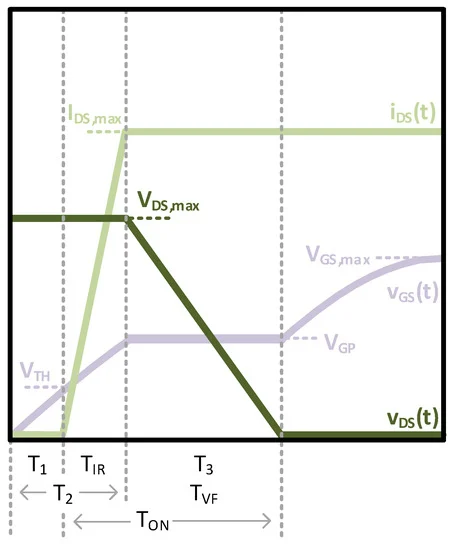
\includegraphics[width=0.7\linewidth]{Bilder/Kapitel2/MOSFET Transient turnon.png}
        \caption{Turn-On Transients}
        \label{fig:MOSFET_transient_turnon}
    \end{minipage}\hfill
    \begin{minipage}{0.5\textwidth}
        \centering
        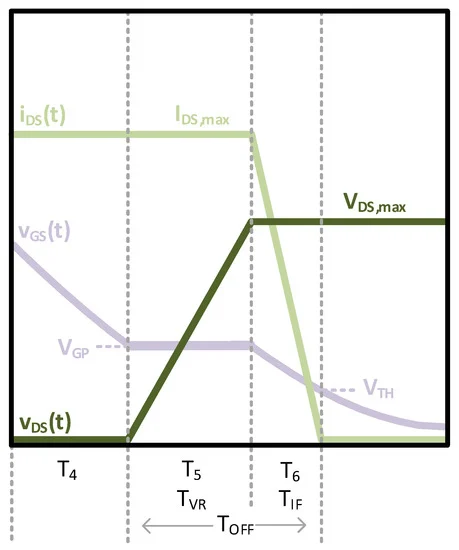
\includegraphics[width=0.7\linewidth]{Bilder/Kapitel2/MOSFET Transient turnoff.png}
        \caption{Turn-Off Transients}
        \label{fig:MOSFET_transient_turnoff}
    \end{minipage}\hfill
\end{figure}
Stepping through the turn-on transient phases, the gate voltage increases, charging the gate-source capacitance $C_{gs}$. As soon as the threshold voltage $V_{th}$ is reached, the \ac{GaNFET} begins to conduct. The gate voltage continues increasing, leading to a rise in the current $I_{ds}$ through the switching element. The drain-source voltage $V_{ds}$ stays constant as the gate-source capacitance $C_{gs}$ is not yet able to discharge through the \ac{GaNFET}. $I_{ds}$ and $V_{gs}$ continue to rise, until the gate-source voltage reaches the miller plateau. At this point, $C_{gd}$ and $C_{gs}$ are effectively connected in parallel, which increases the overall gate capacitance. Furthermore, $C_{gd}$ is charged with a large negative voltage, when compared to $C_{gs}$, resulting in the entire gate current $I_g$ being used to discharge the capacitor. Thereby, $C_{gs}$ cannot continue charging until $C_{gd}$ has reached the same potential. On the other hand, $V_g$ also cannot drop below $V_{pl}$, as this would cause $C_{dg}$ to no longer be able to discharge and $V_g$ to rise to $V_{pl}$ again. As a result, $V_g$ stays constant until $C_{gd}$ has reached the potential of $C_{gs}$. The voltage $V_{ds}$ decreases during this time, as both $C_{gd}$ and $C_{ds}$ are able to discharge. As $V_{ds}$ hits zero, the gate voltage starts to increase again.\\
On turn-off, the same procedure takes place only this time in reverse. The gate voltage $V_g$ decreases as $V_d$ is set to zero until the miller plateau is reached. Here the output capacitances $C_{gd}$ and $C_{ds}$ begin to charge up again, raising the drain-source voltage $V_{ds}$ until they are fully charged. After this, the current begins to drop together with $V_g$ until the threshold voltage $V_{th}$ is reached and the current is equal to zero.\\\\
The energy lost per cycle through turn-on and turn-off is equal to the area of the triangle formed by the product of $V_{ds}(t)$ and $I_{ds}(t)$. Multiplying this by the frequency of cycles $f_s$ gives the total power shown in equation \ref{eq:switching_power}.
The maximum voltages of the transient process are assumed to be constant, since the time of one switching Period $T_s >> t_{on},t_{off}$. For the HS switching element, both at turn-on and turn-off the voltage $V_{ds,max}$ is equal to $V_{in}$. The current, however, differs for the two cases as the inductor current, and thereby the current through the switching element is rising during the on period. At turn-on $I_{ds,max}$ is equal to $(I_{out} - \frac{\Delta I_{L_{pp}}}{2})$ and at turn-off equal to $(I_{out} + \frac{\Delta I_{L_{pp}}}{2})$. Because of this, the total power loss of the HS switching element through switching losses is:
\begin{align}
    P_{s,HS} &= f_s \cdot \frac{1}{2} \cdot V_{ds,max} \cdot I_{in,max} \cdot t_{on,off}\label{eq:switching_power} \\
    &= f_s \cdot \frac{1}{2} \cdot V_{in} \cdot \left[t_{on} \cdot \left(I_{out} - \frac{\Delta I_{L_{pp}}}{2}\right) + t_{off} \cdot \left(I_{out} + \frac{\Delta I_{L_{pp}}}{2}\right)\right]
\end{align}
For the LS switching element, this equation only partially holds, as here the switching does not occur as \textit{hard switching} but as \textit{soft switching}. Ideal \textit{soft switching} comes in the form of \textit{\ac{ZVS}}, \textit{\ac{ZCS}} or a combination of both (ZVZCS). For \ac{ZVS} at turn-on the voltage $V_{ds}$ is discharged before the current begins to rise, effectively creating no region where both $V_{ds}$ and $I_{ds}$ are greater than zero. Since there is no overlap, the power loss is zero, eliminating switching power loss. For turn-off, the same ideal holds for \ac{ZCS}, as letting $I_{ds}$ first drop to zero and then increasing $V_{ds}$ results in zero losses. While ideal soft switching can eliminate switching losses, this is not necessary for something to be considered soft switching. In non-ideal soft switching, the current or voltage is lower than in the hard switching case however, it does not equal zero.\\
This is the case for the \ac{LS} switching element. Since its "body diode", as depicted in figure \ref{fig:GaNFET_ECM}, is pointing in the direction of the current and conducting before turn-on, the voltage $V_{ds}$ is equal to the forward voltage of this "body diode" $V_D$.
\begin{equation}
    V_{ds} = V_D << V_{in}
\end{equation}
Instead of having to lower the voltage from $V_{in}$ to zero during turn-on, it only needs to be lowered from $V_D$, in turn shortening the miller plateau and lowering the product of $I_{ds}$ and $V_{ds}$.
On turn-off, this also holds true, as only $V_D$ needs to be reached. This lowers the switching losses of the \ac{LS} switching element significantly and can therefore be neglected in many cases. To calculate the \ac{LS} switching losses, the same equation \ref{eq:switching_power} as used for the \ac{HS} switching losses is used. Substituting the input voltage $V_{in}$ by the diode voltage $V_D$ and swapping the currents experienced at turn-on and turn-off, yields equation \ref{eq:switching_power_LS}.
\begin{equation}\label{eq:switching_power_LS}
    P_{s,LS} = f_s \cdot \frac{1}{2} \cdot V_D \cdot (t_{on} \cdot (I_{out} + \frac{\Delta I_{L_{pp}}}{2}) + t_{off} \cdot (I_{out} - \frac{\Delta I_{L_{pp}}}{2}))    
\end{equation}
In comparison with the switching losses of the \ac{HS} switching element, here the current at turn-on and turn-off are switched since turn-on for the low side is directly after turn-off of the high side and vice versa for turn-off on the low side.
\subsubsection{Switching element combined losses}
Superposing the discussed types of losses results in a clear frequency dependence. For low switching frequencies, the conductive losses outweigh the dead time and switching losses. At higher frequencies, a linear correspondence between losses and frequency is to be expected. 

\subsection{Losses in the inductor} \label{sec:losses_in_the_inductor}
Concerning inductors, two kinds of losses are differentiated. The losses created by the resistance of the spool are called winding losses, while core losses describe the losses appearing in the core of the inductor. First, the winding losses will be explained, followed by the hysteresis losses of the inductors core.

\subsubsection{Winding losses}
The spool's resistance consists of a base DC resistance which is altered by the frequency-dependent skin effect and proximity effect. The momentary power is then calculated by taking the square of the current through the inductor and multiplying it with this resistance. 
\begin{equation}
    P_{L_{W}}(t) = R(f) \cdot I_L(t)^2
\end{equation}
The average power is then determined by taking the integral of the momentary power and dividing it by the elapsed time.
\begin{equation}
    P_{L_{W}} = \frac{1}{T} \int_{0}^{T} R(f) \cdot I_L(t)^2 dt    
\end{equation}
Losses in the core have two main causes, Eddy currents and Hysteresis. The inductor in the buck converter is subjected to a changing magnetic field. That changing magnetic field induces a voltage in the core, following Faraday's law. According to Lenz's law, this voltage results in a current in the core of the inductor that is opposed to the creating current. These currents form circular paths, hence eddy currents. Considering highly conductive core materials like metal alloys, the low ohmic resistance effectively creates a short and a high current is able to flow resulting in considerate losses. Changing the core material to have a higher resistance, lowering the induced current or splitting the core into many different slices lowering the induced voltage per slice, decreases the core losses resulting from eddy currents. Power inductor cores consisting of powder ferrite or composite materials moulded into the desired shape, provide a high ohmic resistance, as the individual powder particles are insulated from one another.

\subsubsection{Hysteresis losses}
The second type of core loss, hysteresis loss, originates from the core's magnetisation. A non-magnetized core consists of many macroscopic regions of different magnetization. The magnetic moments in one of these regions called magnetic domains are all oriented in the same direction and are separated from the other domains by domain walls only a few hundred atoms wide. When an external magnetic field $H$ is applied to the core, the magnetic domains oriented in the direction of this field expand, shifting the domain walls and increasing the magnetic flux density $B$ in the core. At a certain point, the core becomes saturated, as the domains can only expand further in some regions of the inductor. This explains, why the relationship between the magnetic field strength $H$ and the B-field in an inductor is non-linear. When the current through the inductor and thereby its magnetic field strength decreases, the magnetic flux density also decreases. Depending on the type of core material, the magnetic domains are easy or hard to return to a non-magnetized state. Magnetically hard materials like permanent magnets keep their magnetic flux density even if no external field is present. They have to be subjected to a strong opposing magnetic field, to be demagnitized. On the other hand, magnetically softer materials like steel easily decrease their magnetic flux density, with only a small amount of energy needed to return to a fully demagnetised state. This difference between the charging and discharging behaviour of an inductor is called hysteresis.\\
Plotting the relative B-H curve of an inductor as in figure \ref{fig:b-hcurve} displays this hysteresis, giving insight into the ease of magnetization, point of saturation and the energy stored and released by the inductor. 
The maximum B-field $B_{max}$, the remnant B-field $B_r$ and the coercivity $H_c$ are points of interest along this curve used in later chapters to characterize the inductor.
\begin{figure}[H]
    \centering
    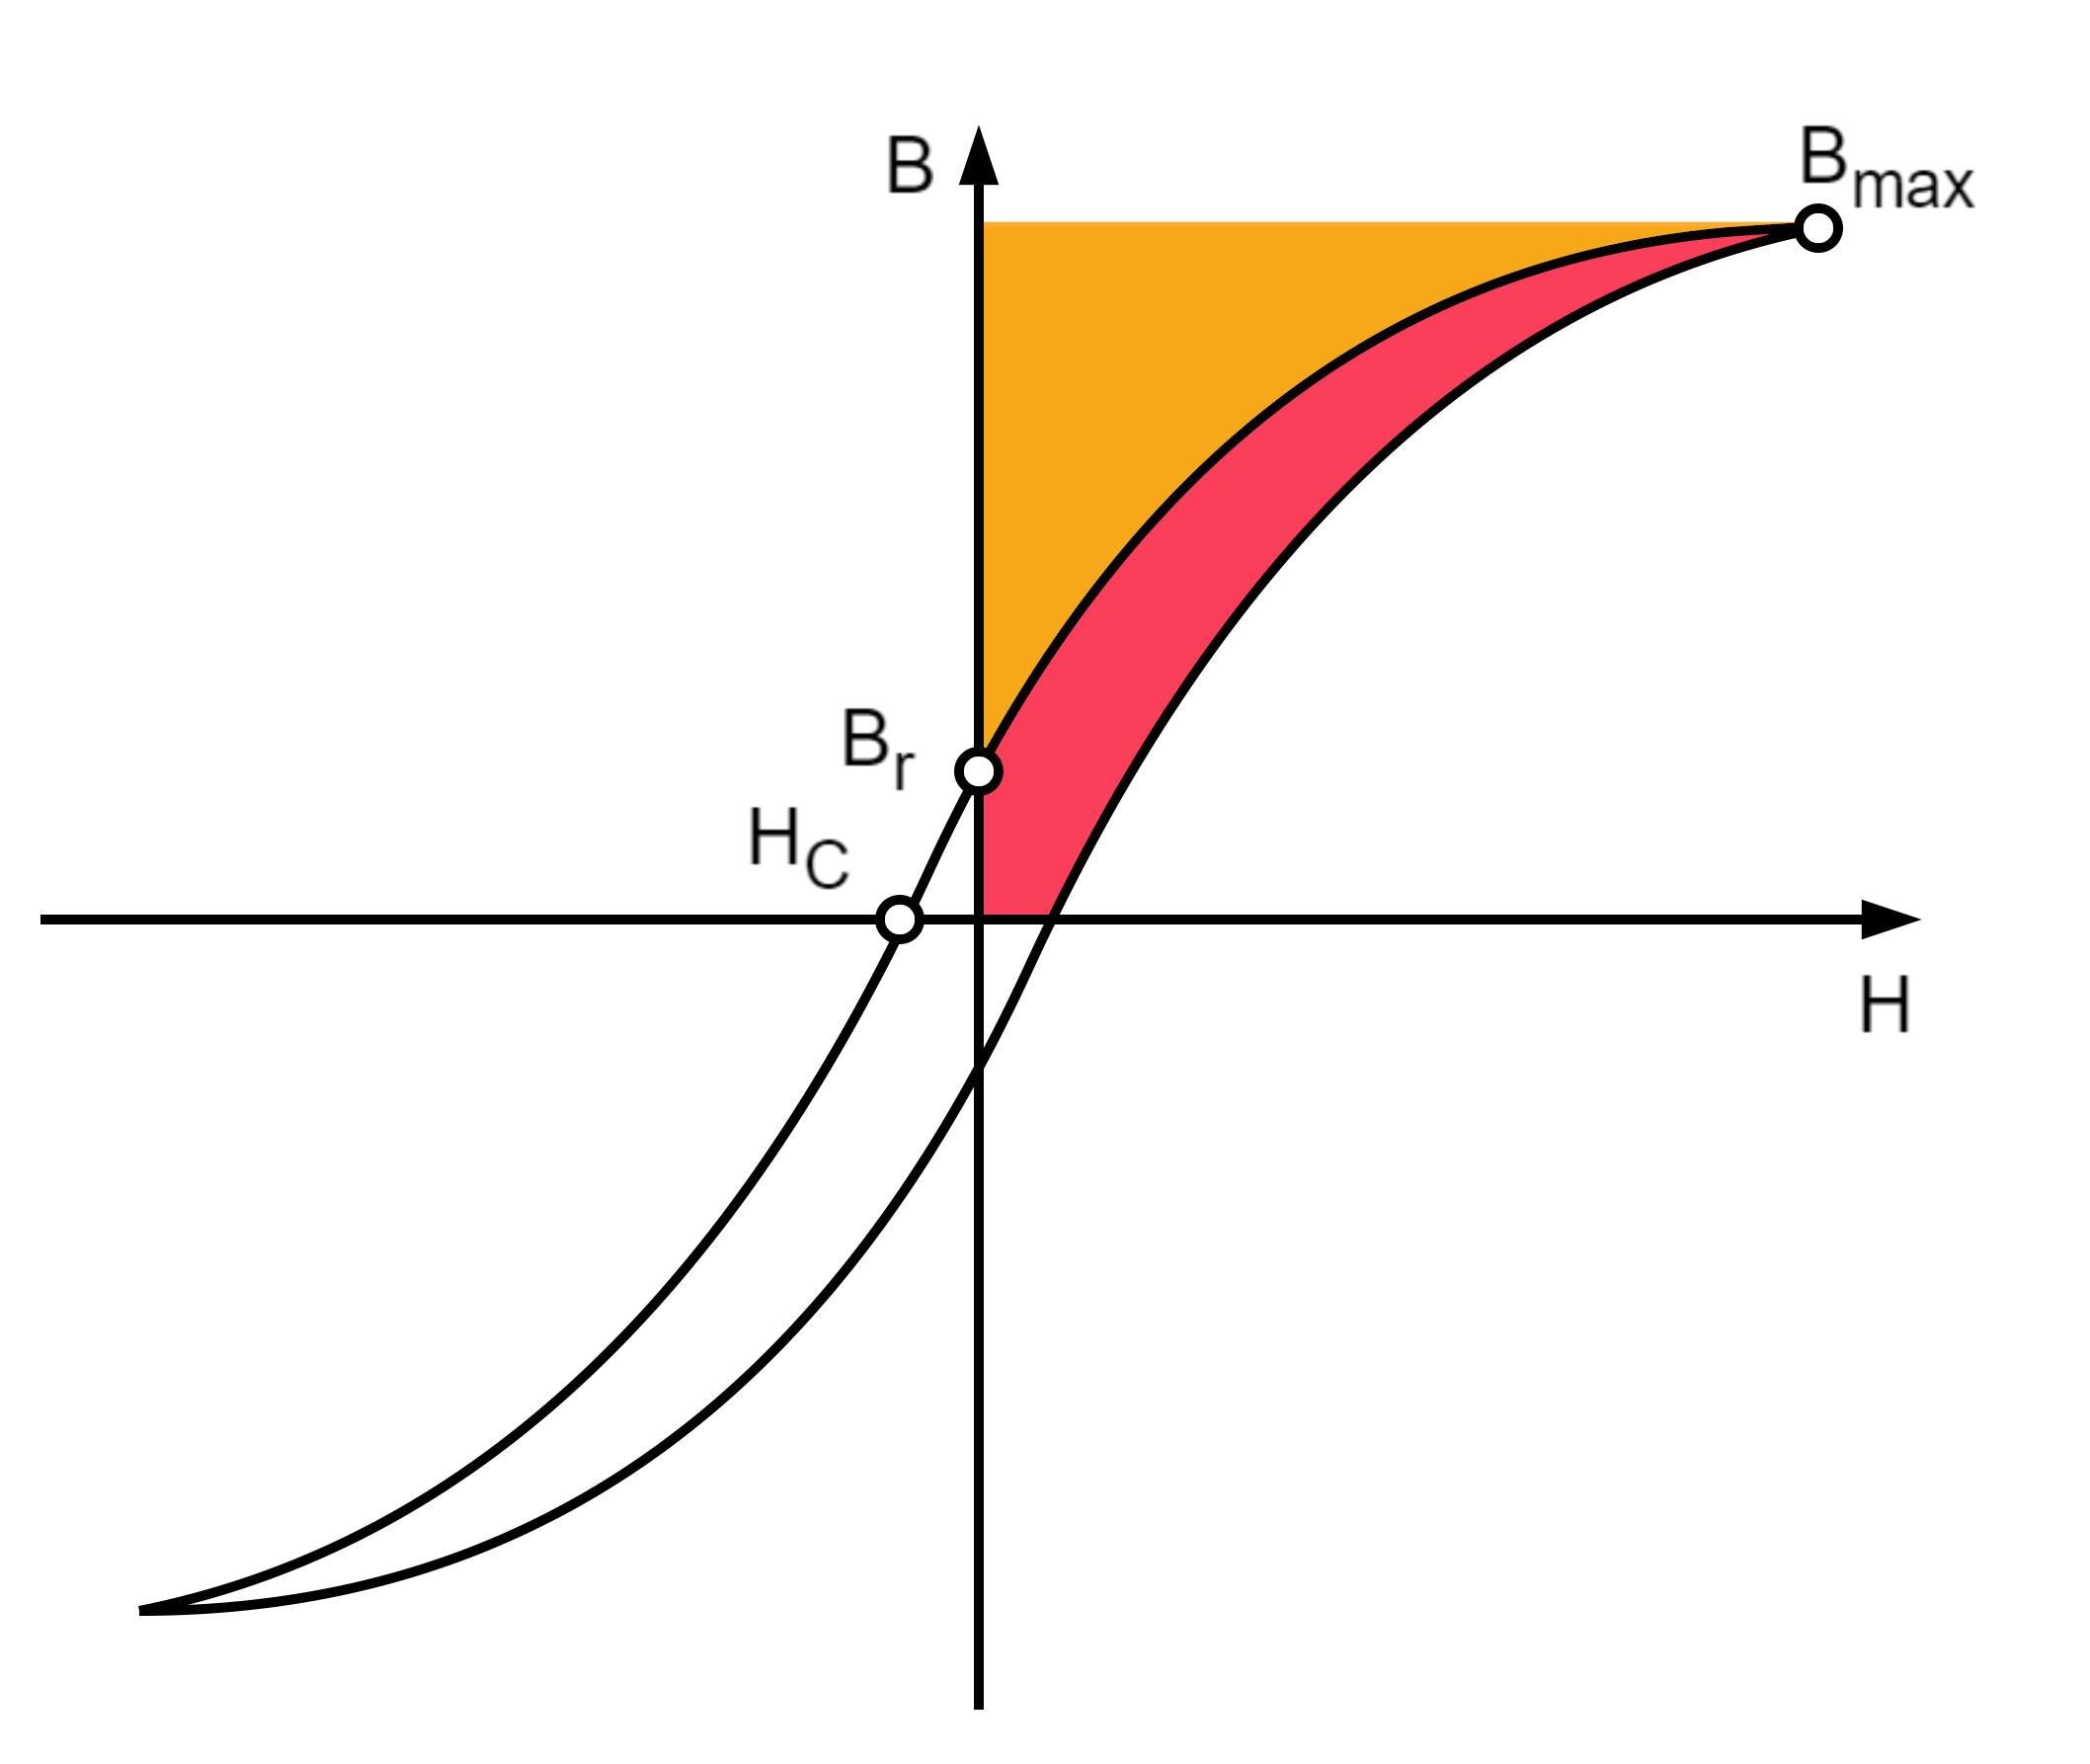
\includegraphics[width=0.6\linewidth]{Bilder//Kapitel2/Hysteresiscurve.png}
    \caption{Hysteresis Loop of a magnetically soft inductor core}
    \label{fig:b-hcurve}
\end{figure}
The energy put into the inductor to charge its B-field can be determined by calculating the area under the curve along the B-field as in equation \ref{eq:hysteresis_energy}. The same equation holds true for the energy released by the inductor when following the upper part of the curve.
\begin{equation}
        E = \int H dB \label{eq:hysteresis_energy}
\end{equation}
The energy lost through charging and discharging the inductor is their difference given as the cyclic integral along the two curves as shown in equation \ref{eq:hysteresis_energy_cyclic}.
\begin{equation}
    E_{loss} = \oint_{Loop} H dB \label{eq:hysteresis_energy_cyclic}
\end{equation}
In buck converters, we assume a constant DC current $I_L$ through the inductor superposed with a ripple current $I_{L_r}$. In accordance with Ampere's Law the momentary H-field is determined by the momentary current through the inductor. Operating with a continuous current through the inductor, the formation of hysteresis loops shown in figure \ref{fig:DC_Bias_Hysteresis} can be observed. 
\begin{figure}[H]
    \centering
    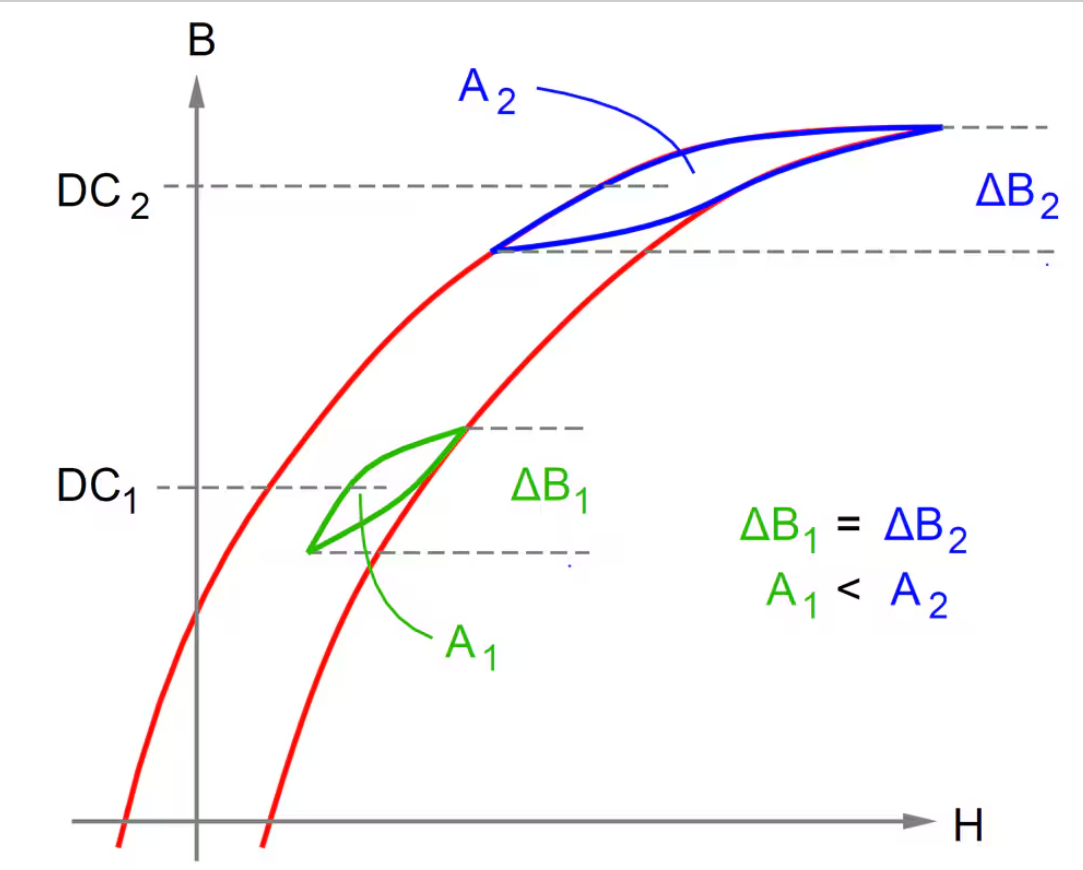
\includegraphics[width=0.4\linewidth]{Bilder//Kapitel2/DC_Bias_Hysteresis.png}
    \caption{Hysteresis Loop with different DC biases}
    \label{fig:DC_Bias_Hysteresis}
\end{figure}
The average H-field is determined by the DC current, while the amplitude of the ripple current determines the difference in the H-field $\Delta H$. The energy lost every cycle of the buck converter is equal to the area enclosed by this loop. The core loss due to hysteresis can therefore be determined by multiplying the area of the loop with the switching frequency.
\begin{equation}
    P_{Hys} = \oint_{Loop} H\left(B,f_s\right)  dB \cdot f_s
\end{equation}
It is important to take into consideration, that the loop size itself is dependent on the switching frequency as the ripple current amplitude is a function of the switching frequency. Therefore, the power lost due to hysteresis is not linearly proportional to the switching frequency, depending heavily on the amplitude of the ripple current.

With a high enough DC current, the inductor reaches saturation. Here, the Inductance $L$ decreases rapidly, increasing the ripple current amplitude and thereby also increasing the size of the hysteresis loop. Operating the buck converter while in saturation is not desirable, as it drastically increases the core losses.

%Herleitung für die Tatsache, dass bei Sättigung der Ripple Current größer wird
%\begin{align}
%    I &= \oint_C H ds = H\cdot\frac{l}{N}\\
%    \Phi &= B \cdot A_c\\
%    L &= \frac{\Phi}{I} = \frac{B}{H} \cdot \frac{N \cdot A_c}{l} \propto \frac{B}{H}\\
%    V_L &= L \cdot \frac{di}{dt} = L \cdot \frac{\Delta i}{\Delta t}\\
%    &\Rightarrow \Delta i \propto \frac{H}{B}
%\end{align}

%This process, called Barkhausen noise, is not continuous but happens in small jumps, as crystal defects, surface defects and further effects impede the domain wall movements. When the impedance is overcome the local magnetisation changes suddenly and a current is induced in the core material. 

%Quelle: 
% https://www.e-magnetica.pl/doku.php/magnetic_saturation#coercivity
% https://www.e-magnetica.pl/doku.php/magnetic_domain
% https://www.e-magnetica.pl/doku.php/domain_wall
% https://ieeexplore.ieee.org/stamp/stamp.jsp?tp=&arnumber=9617451
% https://www.e-magnetica.pl/doku.php/barkhausen_noise





%\section{Characterizing the Inductor}
%Since we are only going up to the first resonant frequency of the inductor, a simple equivalent circuit consisting of a parallel capacitor, two resistors, one in series and one in parallel and the inductor suffices in describing the frequency behaviour of the real inductor.
%\todo[inline]{What can be said about the inductor and how can this be inserted into LT Spice}
%\todo[inline]{Frequencybehaviour}
%\todo[inline]{Saturation}
%\todo[inline]{Hysteresis}




%\subsection{NOTES}
%Skindepth calculations with https://www.allaboutcircuits.com/tools/skin-depth-calculator/ :
%Copper at 4MHz: 32.60um  --> 0.0326mm
%Copper at 80kHz: 230.5um --> 0.235mm
\newpage
\thispagestyle{empty} 
\cleardoublepage

%/Kapitel3
% !TeX root =../main.tex
\chapter{Measuring the Inductor} \label{sec:cha3}
To create a simulated inductor model, first, the characterising parameters of real inductors need to be determined. This chapter presents three measurement approaches, all gathering different data about the inductors in question. The frequency response of the inductors is examined first, with the goal of using the data to create a frequency-dependent impedance to model the inductor's losses for no \ac{DC} bias and small ripple currents. Secondly, the saturation of the inductors is measured to be recreated in LTspice and improve the frequency-dependent model for high \ac{DC} or ripple currents. Lastly, the effects of hysteresis are observed to enable the accurate modelling of \ac{DC} bias and saturation, resulting in a reliable core loss model.\\
The five inductors discussed in this chapter, listed in table \ref{tab:list_of_inductors}, are all products produced by Coilcraft. Falling under the category of power inductors, they are designed to be used in \ac{SMPS} and are therefore common in buck converters. Inductors with similar inductances and core materials were chosen to remain comparable to each other.
\begin{table}[H]
    \centering
    \caption{List of Inductors}
    \begin{tabular}{|c|c|l|}
    \hline
    Inductor &  Inductance & Type \\
    \hline
     XGL1313-103ME & $10 \mu H$ & Molded Inductor \\
        XGL1313-223ME & $22 \mu H$ & Molded Inductor \\
        SER1512-103ME & $10 \mu H$ & High Current Flat Wire Inductor \\
        SER1512-223ME & $22 \mu H$ & High Current Flat Wire Inductor \\
        UA8014-AL & $2 \cdot 10 \mu H$ & Uncoupled Dual Inductors \\
    \hline
    \end{tabular}
    \label{tab:list_of_inductors}
\end{table}

\section{The Frequency Response of the Inductor} \label{sec:the_frequency_response_of_the_inductor}
To accurately measure the inductor's frequency response a "Bode 100" by omicron-lab was used \cite{omicronlabBode100Bode2024}. It functions by subjecting the device under test to a sinusoidal frequency sweep from \SI{1}{\Hz} to \SI{50}{\mega\Hz} and measuring its scattering parameters for every frequency. Each inductor is inserted into the equipment to determine its gain, phase, inductance and \ac{Q-factor}, which are plotted in figure \ref{fig:bode_100_measurements}.\\
Starting out close to purely resistive, the plot shows a shift to inductive behaviour at around \SI{10}{\kilo\Hz}, with magnitude increasing proportional to frequency and the phase approaching \SI{90}{\degree}. At the point of resonance, there is once again a short moment of pure resistive behaviour, after which the inductor begins to act like a capacitor, its magnitude decreasing and phase reaching \SI{-90}{\degree}.\\
\begin{figure}[H]
    \begin{subfigure}[b]{0.50\textwidth}
        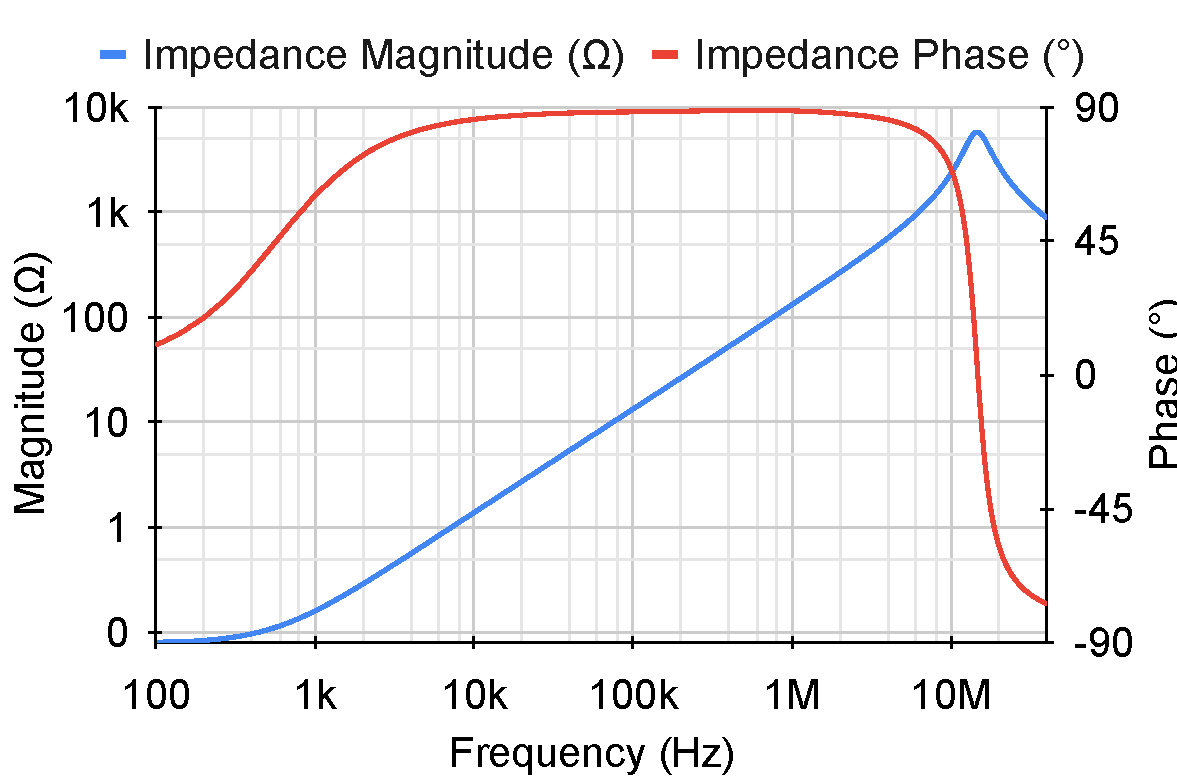
\includegraphics[width=\textwidth]{Bilder/Kapitel3/SER223_BodePlot.pdf}
        \caption{SER1512-223ME complex magnitude and phase vs frequency}
    \end{subfigure}
    \begin{subfigure}[b]{0.50\textwidth}
        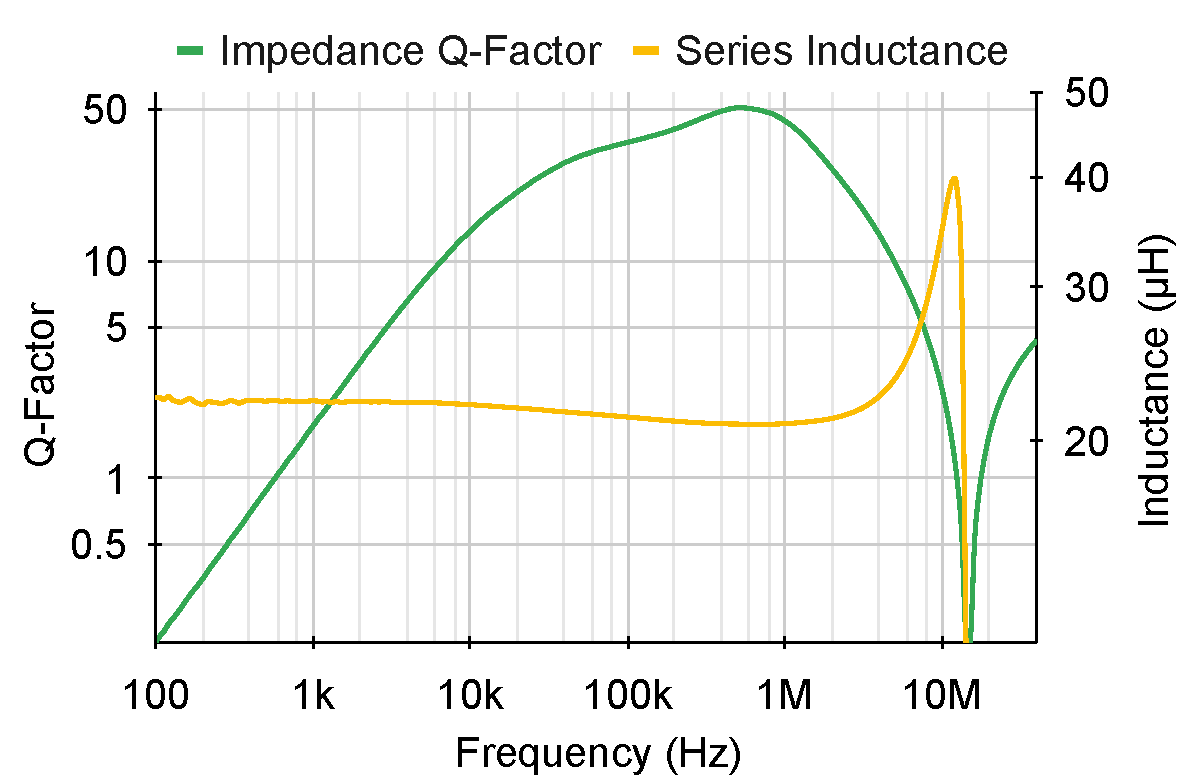
\includegraphics[width=\textwidth]{Bilder/Kapitel3/SER223_QLPlot.pdf}
        \caption{SER1512-223ME \ac{Q-factor} and inductance vs frequency}
    \end{subfigure}
    \caption{Measured frequency response of the SER1512-223ME}
    \label{fig:bode_100_measurements}							
\end{figure}
\section{The Saturation Behaviour of the Inductor} \label{sec:the_saturation_behaviour_of_the_inductor}
To measure the saturation behaviour a "Power Choke Tester" by the manufacturer ed-k was used. It subjects the inductor under test to a rectangular voltage pulse and measures the current through it until a set maximum current is reached. The voltage applied is set to be similar to the actual voltage the inductor is subjected to, here set to \SI{30}{V}. With the voltage and current data, the device is able to calculate the magnetic flux $\Phi$ in the inductor. Calculating the saturation behaviour is done by differentiating the flux.\\ 

The measured saturation behaviours of the \textit{SER1512-223ME}, \textit{UA8014-AL} and \textit{XGL1313-103ME} inductors is displayed in figure \ref{fig:differential_inductance_of_the_ser1512-223me_inductor}. Considering the \textit{SER1512-223ME} inductor, a close to constant inductance with an average of \SI{21.8}{\micro\henry} can be measured up to a current of \SI{5}{\A}, after which the curve decreases following an s-curve. Levelling out at an inductance around \SI{1.18}{\micro\henry}. This means that the inductor enters saturation at around \SI{5}{\A} of \ac{DC} through it, marking this current as the maximum current the inductor should experience without causing the ripple current to increase, resulting in greater power losses.
\begin{figure}[H]
    \centering
    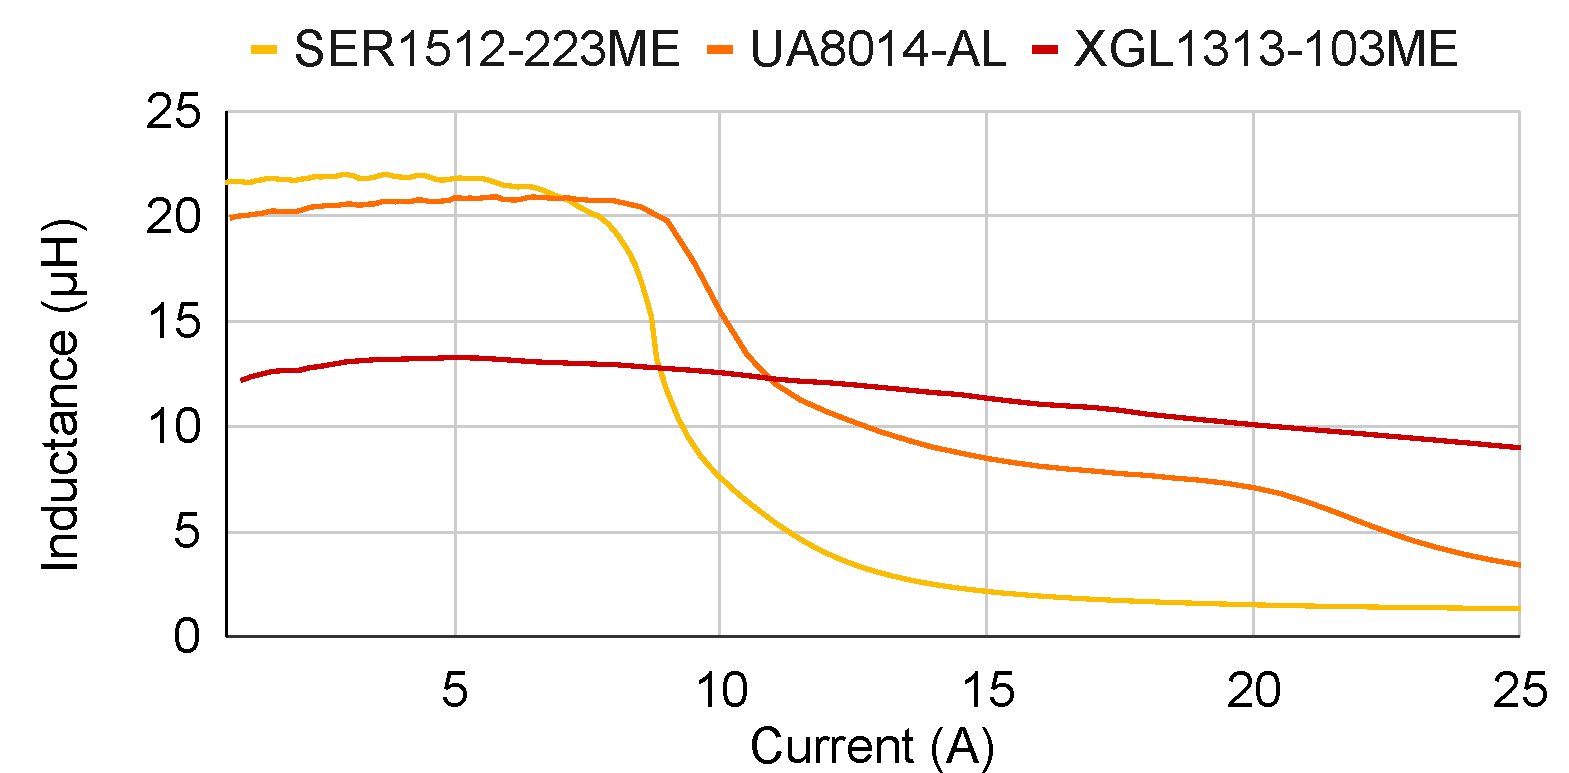
\includegraphics[width=0.8\linewidth]{Bilder//Kapitel3/SER223_UA_XGL103_Saturation.pdf}
    \caption{Differential inductance of the SER1512-223ME and UA8014-AL inductor}
    \label{fig:differential_inductance_of_the_ser1512-223me_inductor}
\end{figure}
The difference in the behaviour of this inductor to the \textit{XGl1313-103ME} inductor can be led back to two reasons. Firstly the \textit{XGL}-inductor is only a \SI{10}{\micro\H} inductor, compared to the \SI{22}{\micro\H} \textit{SER}-inductor, explaining their different initial inductances. Secondly, the very gradual reduction of the saturation of the \textit{XGL}-inductor is a direct consequence of its air gap. As stated in section \ref{sec:the_working_principal_of_the_inductor}, the air gap stretches the saturation graph, leading to a more gradual decline in the inductance and increasing the saturation current.
Being made from composite materials, instead of a ferrite, the \textit{XGL1313-103ME} does not contain a direct gap in the inductor's core. Rather the density of paramagnetic material in the composite powder is charged for different sections of the core material, creating an air gap distributed throughout some parts of the core.

\section{The Hysteresis Behaviour of the Inductor}
In order to measure the hysteresis behaviour of an inductor, the magnetic field $H$ and the magnetic flux density $B$ at any moment in the inductor's charge cycle need to be calculated, as they cannot easily be measured directly. By using Ampere's law of equation \ref{eq:amperes_law} the magnetic field $H$ can be determined by measuring the current through the inductor and 
with the help of the magnetic length $l_m$ and the number of windings $N$.
\begin{equation}\label{eq:amperes_law_toH}
    H = I \cdot \frac{N}{l_m} 
\end{equation}
Similarly, the voltage across the inductor is used to calculate the magnetic flux density $B$, making use of Faraday's law given in equation \ref{eq:faradays_law}. It rearranges to 
\begin{equation}\label{eq:faradays_law_toB}
	B = \frac{1}{N \cdot A_c} \int_0^t v(\tau)d\tau \quad\text{.}   
\end{equation}
Both equations rely on exact measurements of the inductor's magnetic length $l_m$ and crossectional area $A_c$. These measurements are often not provided by the inductor manufacturer, as is the case with all inductors examined in this thesis. To provide a proof of concept of the measurement setup, a custom wound inductor with known core parameters is used. The chosen core from the producer ferroxcube, called PQ20/16 \cite{ferroxcubeMaterialSpecifications3C952015, ferroxcubeProductSpecificationsCore2016}, came with exact values for each of the unknown parameters and a measured hysteresis curve. It provides a direct control to validate the measurement approach while eliminating errors in the measurement of the core's dimensions. The core is wound with 8 windings and pressed together to create an inductor without an air gap. Hereby all variables for the hysteresis measurement are known.
\begin{table}[H]
    \centering
    \caption{Parameters of the custom inductor \cite{ferroxcubeMaterialSpecifications3C952015}}
    \begin{tabular}{|l|c|c|c|c|}
        \hline
        Parameter & Magnetic length $l_m$ &  Air gap length $l_g$ &  Effective area $A_e$ & Windings $N$ \\
        \hline
        Value & \SI{37.8}{\milli\m} & \SI{0}{\milli\m} & \SI{61.9}{\milli\square\m} & 8\\
        \hline
    \end{tabular}
    \label{tab:parameters_of_the_custom_inductor}
\end{table}

Measuring the hysteresis is done by subjecting the inductor under test to a rectangular voltage pulse until the core reaches saturation. After that the voltage is dropped and the inductor discharges on its own. Since there was no dedicated device available, the setup displayed in figure \ref{fig:hysteresis_measurement_setup} needed to be implemented manually.
\begin{figure}[H]
    \centering
    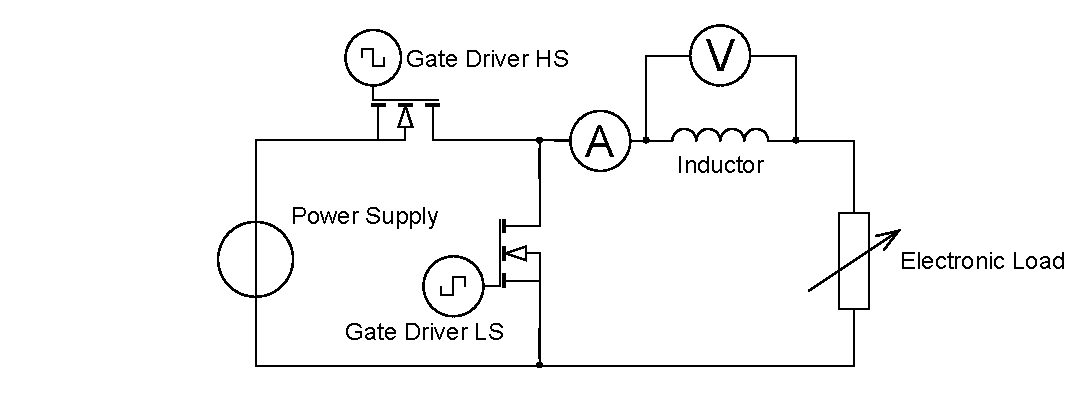
\includegraphics[width=1\linewidth]{Bilder/Kapitel3/Hysteresis_Measurement_Setup.pdf}
    \caption{Hysteresis measurement setup}
    \label{fig:hysteresis_measurement_setup}
\end{figure}
Using a \ac{GaNFET} half-bridge to connect the inductor to and adding a load with capacitive and resistive properties, allows the charging time to be regulated and a reverse current to flow through the inductor. The reverse current is necessary to measure the coercive force $H_c$. Connecting a current clamp to the wire leading to the inductor and a voltage probe across the inductor enables the oscilloscope to measure the hysteresis curve. As the voltage supplied to the inductor determines the rate of change of the inductor current, a lower switching frequency is desirable, as it allows a lower voltage to be used to achieve the same maximum current since more time for the charging process is given.\\
Limiting factors of this setup are the minimum speed the \ac{GaNFET} half-bridge can switch at, the maximum change in current the power supply can deliver and the maximum power spikes the electronic load is able to handle. In this case, the minimum switching speed achieved was \SI{10}{\kilo\Hz}, which is just low enough to enable a clear measurement.\\

Inserting the custom inductor into the measurement setup shown in figure \ref{fig:hysteresis_measurement_setup}, applying a \SI{52}{\V} supply voltage, allowing a maximum \SI{30}{\A} current pull and switching at \SI{13}{\kilo\Hz}, the behaviour shown in image \ref{fig:hysteresis_measurement_of_the_custom_wound_inductor} was created. 
Hysteresis and saturation behaviour are clearly visible. The noise in the measurements at the points where the axes are crossed is not negligible, influencing the values of the remnant B-field $B_r$ and the coercivity $H_c$. Most of this noise is a product of measurement noise, as the oscilloscope needs to measure high voltages and currents, which worsens the resolution at low currents and voltages. The distortion visible at the maximum point of saturation is due to fluctuations in the voltage of the power supply, as it operates at its peak capabilities.
\begin{figure}[H]
    \centering
    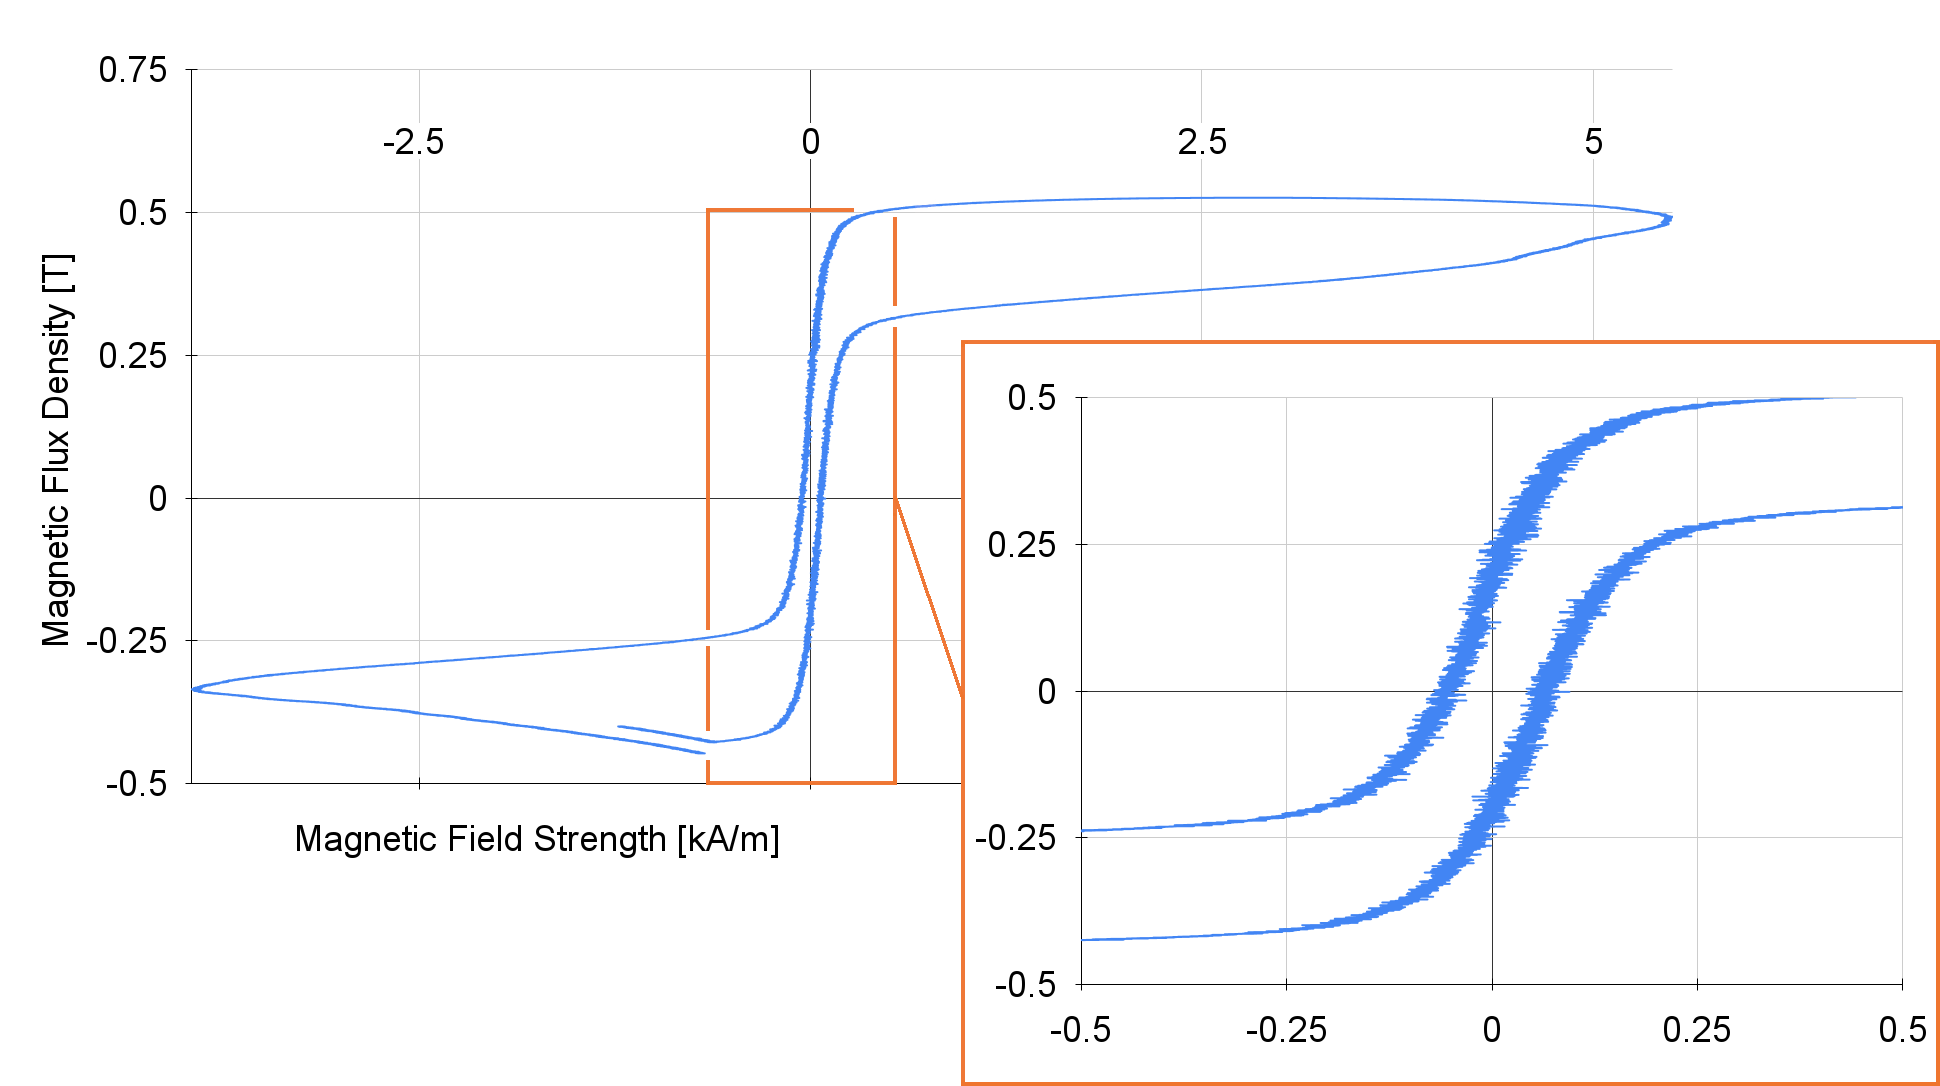
\includegraphics[width=1\linewidth]{Bilder//Kapitel3/Hysteresis_Measurement_3.png}
    \caption{Hysteresis Measurement of the custom wound inductor}
    \label{fig:hysteresis_measurement_of_the_custom_wound_inductor}
\end{figure}
Table \ref{tab:B-H_curve_points_of_interest_comparison} compares the measured points of interest to the data provided by the producer of the core material. While the deviations are noticeable, they are still attributable to the noise and limitations of the setup. If the setup is changed to allow for higher precision at low currents and voltages and the saturation region is not plagued by unwanted behaviour of the power supply and electronic load, the results can be improved. This validates the use of this approach to also measure inductors, whose core parameters are unknown. First, however, the measured results are imported into LTspice to determine the validity of the model in the following chapter.
\begin{table}[H]
    \centering
    \caption{Comparison of B-H curve parameters \cite{ferroxcubeProductSpecificationsCore2016}}
    \begin{tabular}{|l|c|c|}
        \hline
        & Measured & Given by the data sheet \\
        \hline
        Coercive Force $H_c$ & \SI{54}{\A\per\m} & \SI{13}{\A\per\m}\\ 
        \hline
        Remnant B-Field $B_r$ & \SI{255}{\milli\tesla} & \SI{156}{\milli\tesla}\\
        \hline
        Maximum B-Field $B_{max}$ & \SI{570}{\milli\tesla} & \SI{500}{\milli\tesla}\\
        \hline
    \end{tabular}
    \label{tab:B-H_curve_points_of_interest_comparison}
\end{table}




















\newpage
\thispagestyle{empty} 
\cleardoublepage

%/Kapitel4
% !TeX root =../main.tex
\chapter{Implementation and Validation of the Inductor in LTspice} \label{sec:cha4}
In this chapter, the measurements of the previous chapter are used to create a simulated inductor model in LTspice. The goal: create a mixture of these to best recreate the reality of the inductor's behaviour. Again, three different approaches are taken, each mapping directly to one of the phenomena measured in chapter \ref{sec:cha3}. In each case, the used model is introduced first, followed by the steps taken to include the measured data in the model. The models are then separately simulated in different configurations and validated using available data. 

\section{Modeling the Frequency Response of the Inductor} \label{sec:modeling_the_frequency_response_of_the_inductor}
The first and simplest type of inserting non-idealities into the inductor Model of LTspice is with an \ac{ECM}. It can simulate the frequency response of a real inductor. The base inductor already has an \ac{ECM} pictured in figure \ref{fig:inductor_ecm}, taking into account the equivalent parallel capacitance between the individual windings of the inductor $EPC$, the copper resistance at low frequencies $ESR$ and the overall resistance during resonance $EPR$. It acts as a starting point to approximate the frequency response of an inductor and as later demonstrated, is enough to characterise the studied inductor's frequency response fully.
\begin{figure}[H]
    \centering
    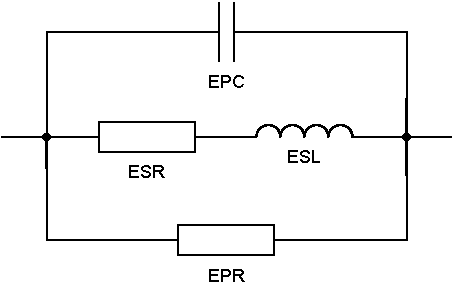
\includegraphics[width=0.5\linewidth]{Bilder//Kapitel3/Inductor_ECM.pdf}
    \caption{Inductor \ac{ECM}}
    \label{fig:inductor_ecm}
\end{figure}
Using the resulting graphs of section \ref{sec:the_frequency_response_of_the_inductor}, all four parameters of the \ac{ECM} can quickly be determined. The series resistance is equal to the magnitude of the impedance at its lowest frequency. Even though the phase at this point still isn't zero and therefore inductive properties remain, the approximation still holds true, as both magnitude and phase level out before this point. The inductance is determined similarly and can be read from the series inductance graph for low frequencies. Parallel capacitance and resistance are determined by the point of resonance. For the \textit{SER1512-223ME} inductor, the resonant point lies at \SI{14,725}{\mega\Hz} with a pure resistance of \SI{5,582}{\kilo$\Omega$}. This resistance defines the parallel resistance of the \ac{ECM}. For the parallel capacitance, the point of resonance is used, as the inductive reactance and capacitive reactance are equal in magnitude. Rearranging this equation, the capacitance can be determined by
\begin{equation}\label{eq:ecm_capacitance}
    C_P = \frac{1}{\left(2 \pi \cdot f_r\right)^2\cdot L} \quad\text{\cite{bitschnauPowerInductorModelling}.}
\end{equation}
Simulating the frequency response in LTspice is done by connecting the inductor model to a current source set to \ac{AC} analysis, mirroring the operation of the "Bode 100". The current source sweeps the chosen frequency range with a sinusoidal current with an amplitude of \SI{1}{A}. Measuring the voltage across the entire equivalent circuit after running an \ac{AC} simulation yields the frequency response of the inductor. Since the amplitude and phase of the voltage are determined by the product of the frequency-dependent impedance and the current, which is always \SI{1}{A} with a \SI{0}{\degree} angle, the complex measured voltage value equals the responding impedance value $Z_L$ at that frequency. The \ac{Q-factor} gives insight into how well the inductor is approximating an ideal inductor, showing a range for the optimal operating frequency for the inductor considering pure sinusoidal excitation. It is calculated by
\begin{equation}
    Q = \frac{Im(Z_L)}{Re(Z_L)} \quad\text{.} 
\end{equation}
The inductance simply is the imaginary part of the impedance, divided by the angular frequency up until resonance, as after that the inductor behaves like a capacitor. 
\begin{figure}[H]
    \begin{subfigure}[b]{0.50\textwidth}
        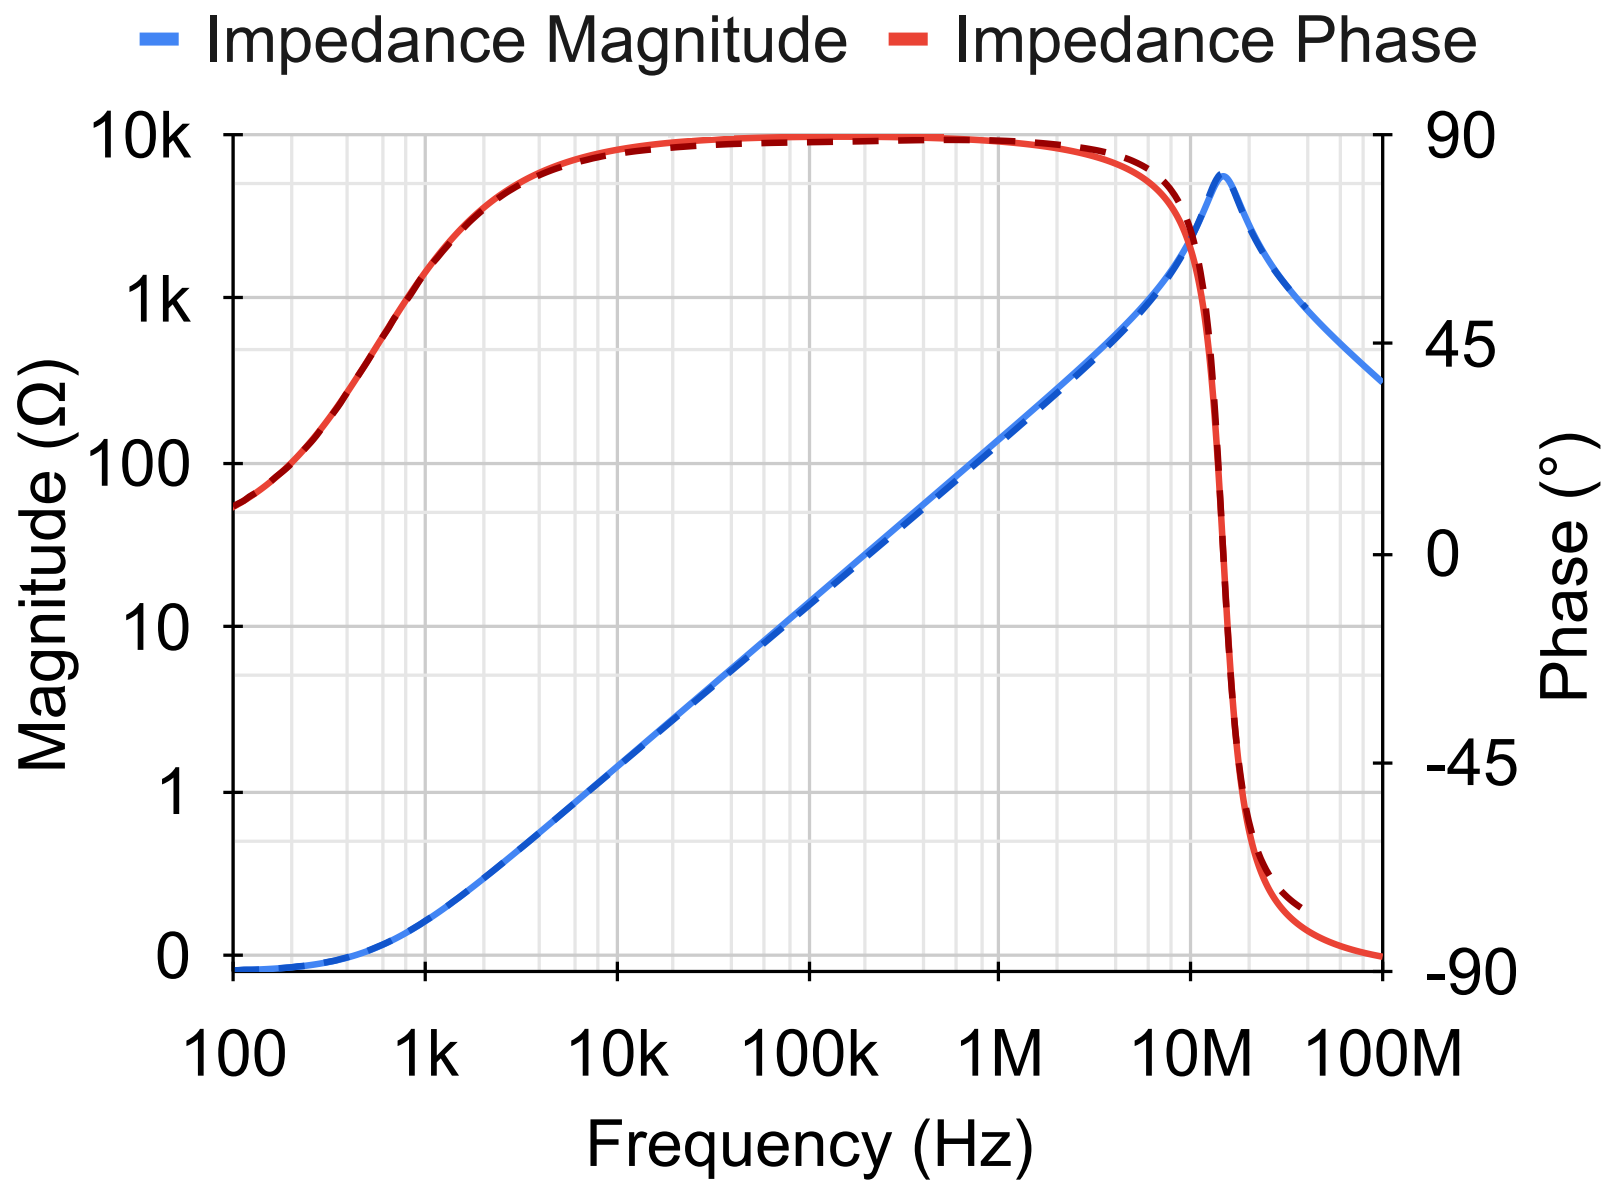
\includegraphics[width=\textwidth]{Bilder/Kapitel3/SER223_BodePlot_Combined.png}
        \caption{SER1512-223ME complex magnitude and phase vs frequency}
    \end{subfigure}
    \begin{subfigure}[b]{0.50\textwidth}
        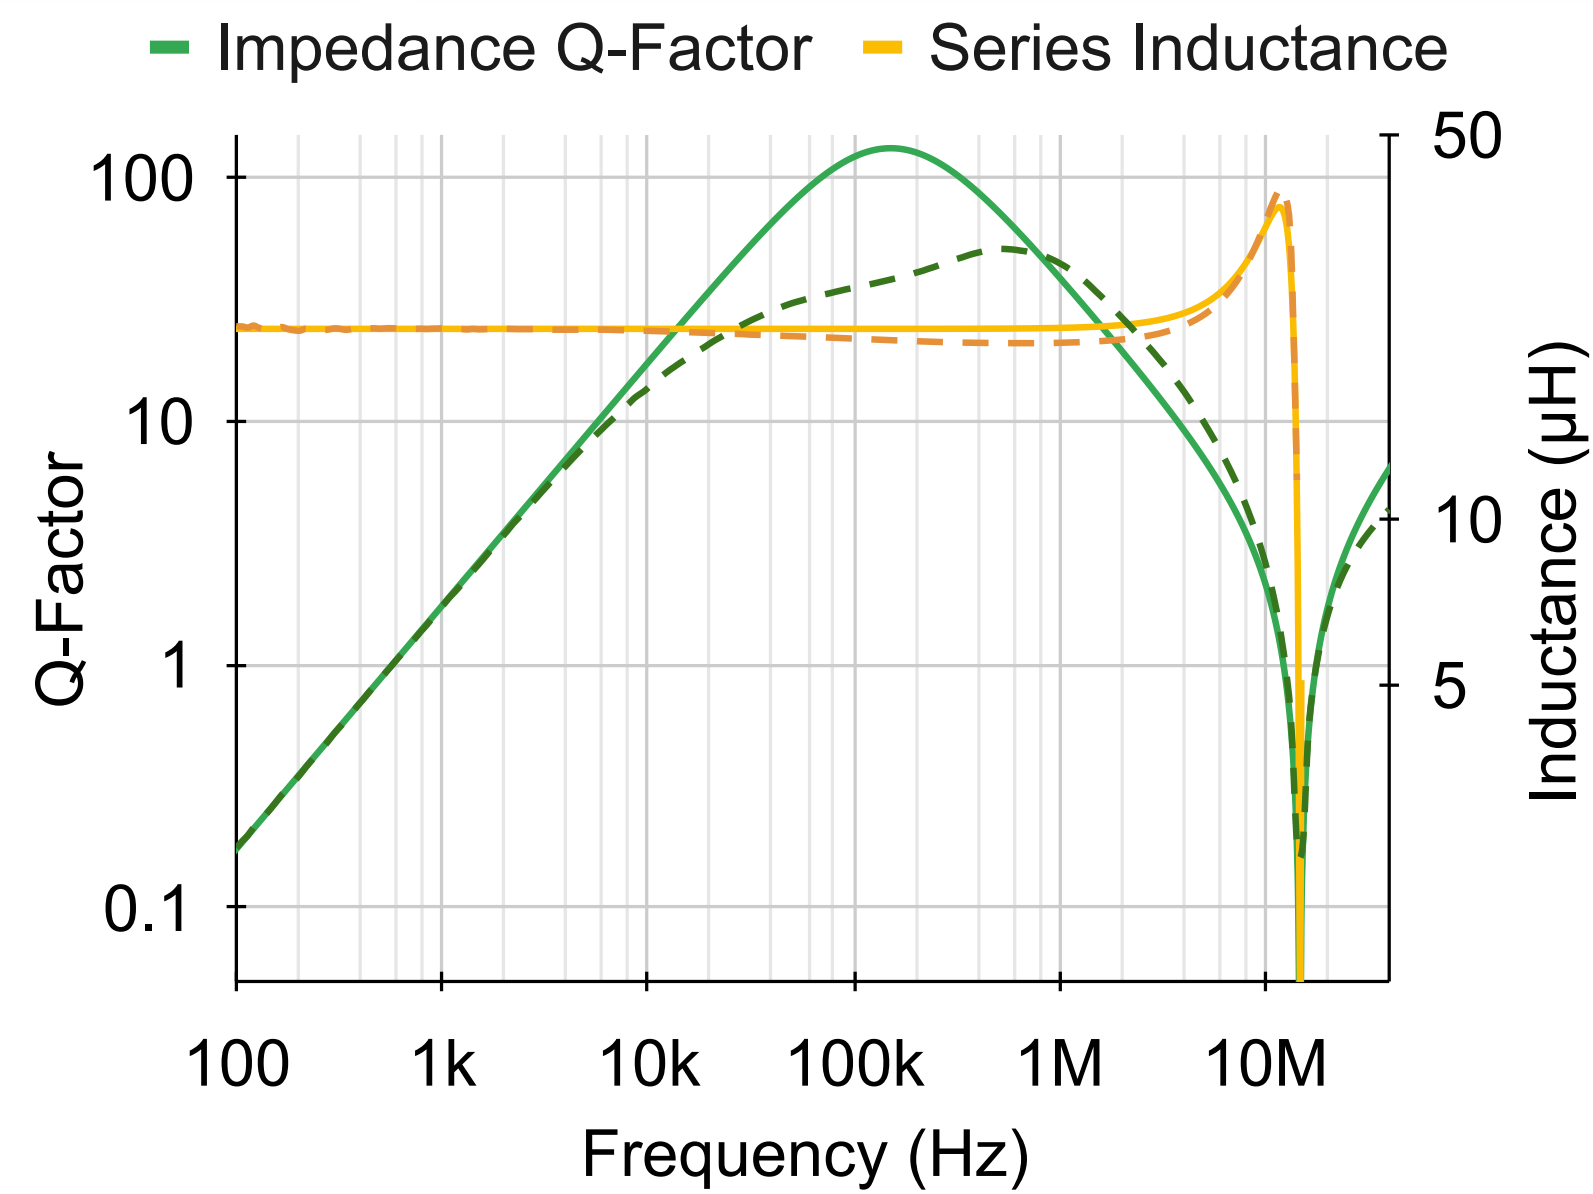
\includegraphics[width=\textwidth]{Bilder/Kapitel3/SER223_QLPlot_Combined.png}
        \caption{SER1512-223ME \ac{Q-factor} and inductance vs frequency}
    \end{subfigure}
    \caption{Simulated and measured frequency response of the SER1512-223ME\\striped lines indicate measured values, while continuous lines are simulated}
    \label{fig:bode_100_measurements_combined}							
\end{figure}
Overlaying the results of the measurements and the LTspice simulation in figure \ref{fig:bode_100_measurements_combined}, the \ac{ECM} closely models the true frequency response, justifying its use. While impedance magnitude and phase match close to perfectly, the \ac{Q-factor} and inductance slightly stray from the true values. Since the \ac{Q-factor} is sensitive to small changes in the imaginary part of the impedance its deviation from the measurement can be attributed to the slight frequency dependence of the measured inductance. The small change of the inductance before resonance is not separately modelled in the simulation \ac{ECM}, leading to the error in the \ac{Q-factor}.
Using this approach, all five inductors were modelled and implemented in LTspice with similar results to the ones presented. The results of figure \ref{fig:bode_100_measurements} show, that the frequency response of the simulated inductor is able to fully recreate the frequency behaviour of the physical inductor.

\section{Modeling the Saturation Behaviour of the Inductor}\label{sec:modeling_the_saturation_behaviour_of_the_inductor}
The second type of inductor loss modelling takes advantage of the LTspice inbuilt \textit{flux} function. With it, a specific saturation curve can be input into the inductor, modelling the current dependence of the inductance. Since this model does not influence the frequency behaviour of the inductor, it is used in combination with the results from the previous section, only replacing the inductor of the \ac{ECM} by the \textit{flux} function.\\
The validation of the model takes place in two steps. To start with, the saturation measurement is recreated in LTspice to measure the simulated saturation curve. Following this, the model is subjected to the excitation of a buck converter where the ripple current's amplitude $\Delta I_{L_r}$ is compared for different \ac{DC} biases. 

To represent the current behaviour of the inductance in the simulation, the measured data needs to be imported. Directly importing the measured flux from section \ref{sec:the_saturation_behaviour_of_the_inductor} value by value into LTspice is no option, as both the number of values LTspice able to be stored is limited and the runtime of the simulation is drastically increased. Instead, curves are fitted to the saturation measurements that best describe the inductance for each inductor. A combination of different degree polynomials and exponential functions define a piecewise function that approximates the saturation behaviour of the inductance. Integrating this function yields the flux curve, which can then be imported into LTspice using the \textit{flux}-command of the inductor.

\subsection{Validation by Saturation Behaviour}\label{sec:validation_by_saturation}
Measuring the inductance curve in the simulation is done by subjecting the inductor to an \ac{AC} with an amplitude of $\frac{1}{2\pi}$\SI{ }{\A}, frequency of \SI{1}{\Hz} and a varying \ac{DC} offset. The chosen values enable the inductance to be determined by measuring the voltage across the inductor. As the inductor's voltage is the product of the \ac{AC} amplitude and the inductor's complex impedance, the frequency factor of $2\pi$ and the current's amplitude cancel out, resulting in the voltage being numerically equivalent to the inductance.
\begin{equation}\label{eq:inductance_from_voltage}
    \hat{V}_L = \hat{I}_L \cdot j 2\pi f\cdot L \triangleq L
\end{equation}
Comparing the inductance curve of the \textit{UA8014-AL} inductor when measured and simulated, the flexibility and precision of this approach can be well demonstrated. The fitted curve, consisting of many piecewise-defined functions, is able to closely follow the measured inductance. While sensibly extending the inductance curve for values close to \SI{0}{\A} of current, high-frequency measurement noise is also removed, visible in the low amperage range of the measured inductance curve. Furthermore, it has the advantage of causing no noticeable increase to the simulation runtime when compared to a model without the \textit{flux}-command utilised. 
\begin{figure}[H]
    \centering
    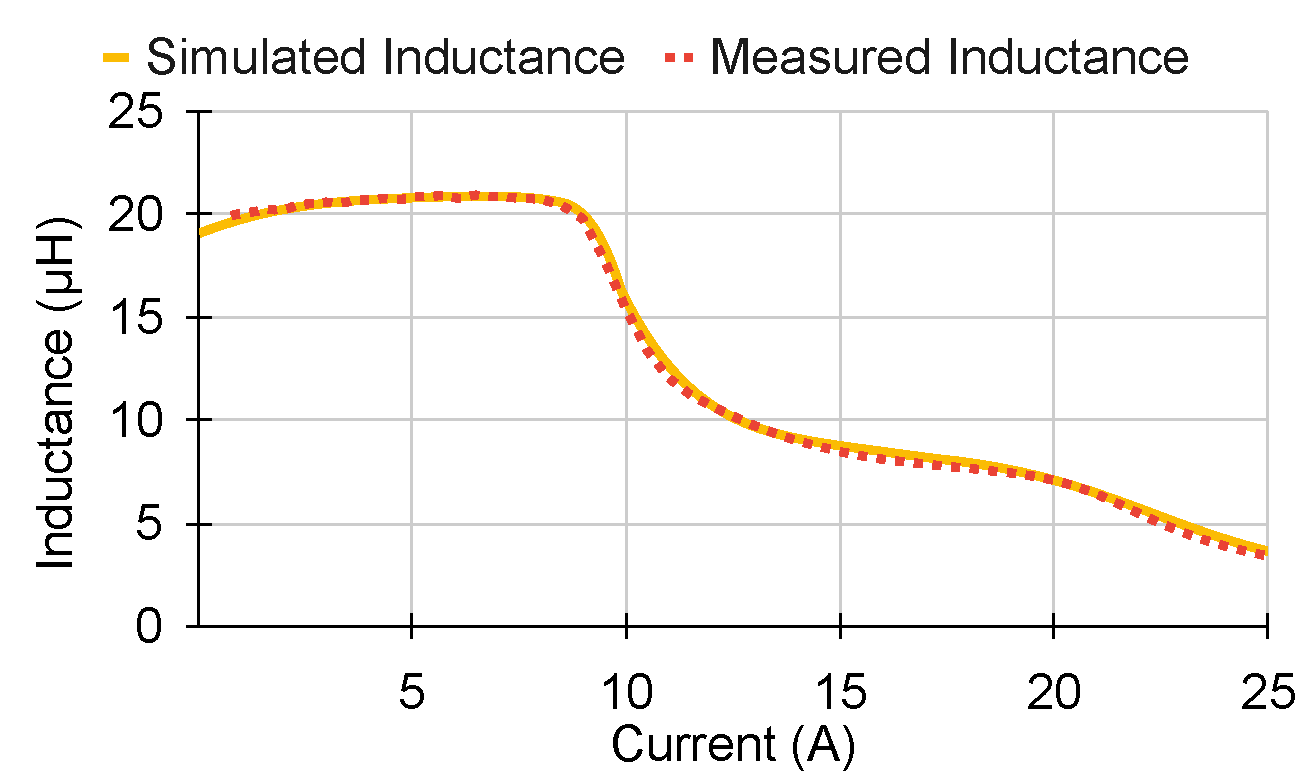
\includegraphics[width=0.7\linewidth]{Bilder/Kapitel3/Saturation_Measured_vs_LTspice.pdf}
    \caption{Comparison of the Inductance curve of the \textit{UA8014-AL} measured and simulated}
    \label{fig:comparison_of_saturation}
\end{figure}
\subsection{Validation by Ripple Current Amplitude}\label{sec:validation_by_ripple_current_amplitude}
To test the viability of the saturation model in a buck converter, the behaviour of its ripple current amplitude for different \ac{DC} bias currents is examined.\\

Simulating the inductor is done by connecting the model to a pulsing voltage source and constant current load. The voltage source simulates the excitation caused by the switching elements, without using direct \ac{GaNFET} models. This ensures that all effects are purely based on the inductor. To enable a ripple current to flow, a capacitor is also added in parallel to the current source, completing the circuit diagram shown here.
\begin{figure}[H]
    \centering
    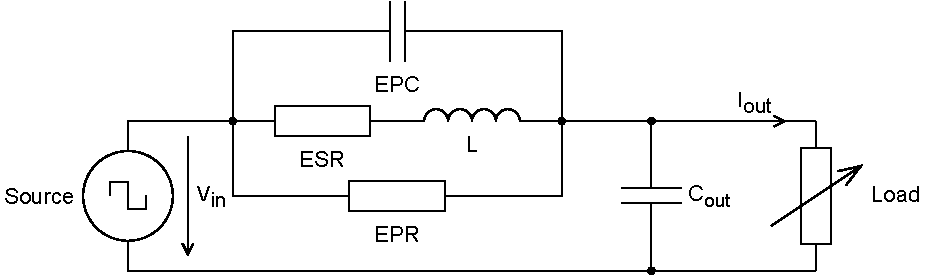
\includegraphics[width=1\linewidth]{Bilder/Kapitel4/Saturation_Validation_ECM.pdf}
    \caption{Circuit Diagram simulating the behaviour of a buck converter}
    \label{fig:saturation_validation_circuit_diagramm}
\end{figure}
The voltage source sends out rectangular voltage pulses with a 50\% duty cycle, \SI{30}{\V} peak at a switching frequency of \SI{300}{\kilo\Hz}. Measuring the peak-to-peak amplitude of the ripple current flowing through the \ac{ECM}, the current drawn by the simulated load is increased step by step from \SI{0.5}{\A} to \SI{20}{\A}. This process is then repeated for all five inductors. For the physical measurements, a buck converter with the same inductors is used. Its output current $I_{out}$ is also increased up to \SI{20}{A}.\\

Observing the measured data of the physical buck converter, a \ac{DC} dependent increase of the ripple currents amplitude is detected for all inductors. This increase, however, is not uniform between the inductors. For the \textit{SER1512} inductors, their ripple current scales up drastically, as soon as the approximate saturation current of \SI{7}{\A} and \SI{10}{\A} is reached. At \SI{20}{\A} \ac{DC} both register a peak-to-peak ripple current amplitude of more than \SI{15}{\A}. In comparison, the \textit{XGL1313} inductors only increase their ripple current amplitude slightly after reaching saturation.\\\\
\begin{figure}[h]
    \centering
    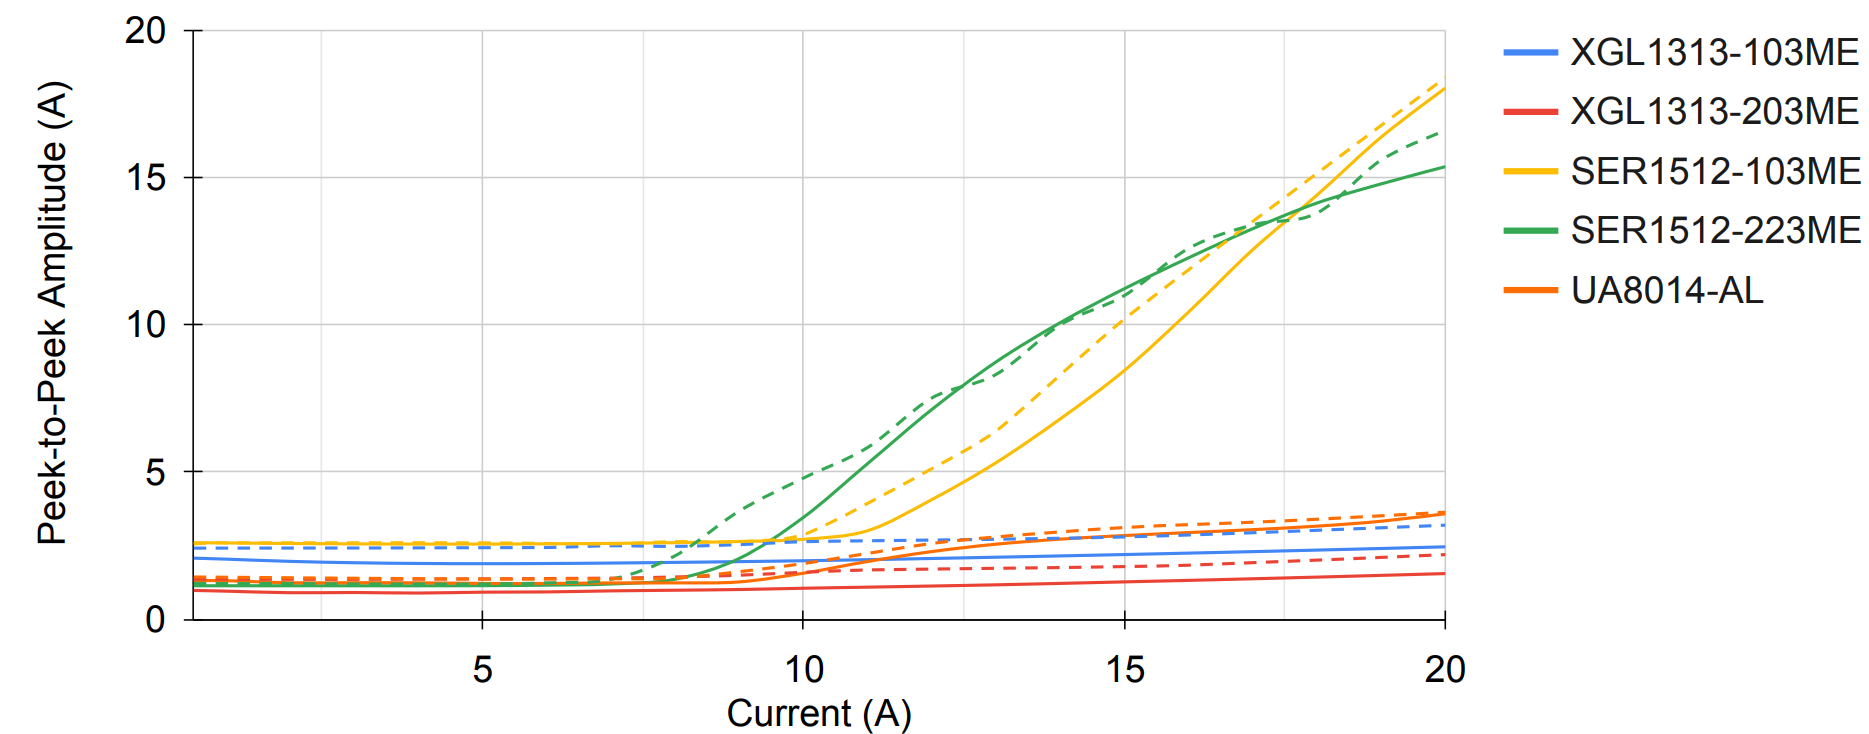
\includegraphics[width=1\linewidth]{Bilder//Kapitel4/High Current_2.png}
    \caption{Ripple current amplitude for high currents \\striped lines indicate measured values, while continuous lines are simulated}
    \label{fig:ripple_current_amplitude_for_high_currents}
\end{figure}
This behaviour mirrors the measured saturation curves. As seen in figure \ref{fig:comparison_of_saturation} the \textit{SER1512} experience a large inductance drop at saturation, while the \textit{XGL1313} gradually decrease their inductance due to a larger air gap. This causes the ripple current amplitude for a high \ac{DC} through the \textit{XGL1313} inductors, to not increase as drastically, as for the \textit{SER1512} inductors.\\\\
Regarding the simulated peak-to-peak amplitudes, their global behaviour reflects the behaviour of the real inductor well. For the inductors with a sharp inductance drop, their ripple current amplitude in the simulation increases rapidly too, while for the inductors with a gradual inductance decrease, their ripple current amplitude also increases gradually. While discrepancies are present, these are expected due to two main reasons. Firstly measurement errors in the peak-to-peak amplitudes of the physical buck converter introduce noise, most clearly seen for inductor \textit{SER1512-223ME}. Secondly, the saturation model is not able to represent the effects of \ac{DC} bias in the physical inductors. But even though this effect is not represented, the saturation model stays valid for both low currents, where saturation is not a factor, as well as high currents, where \ac{DC} bias has its greatest effect. \\

\section{Modeling the Hysteresis Behaviour of the Inductor}\label{modeling_the_hysteresis_behaviour_of_the_inductor}
The third type of LTspice inductor modelling examined is hysteresis modelling. In contrast to the saturation model, it takes the \ac{DC} bias into account with the hope of modelling the inductor behaviour at high output currents accurately.\\
In contrast to the flux, where a function can be directly input in LTspice, the hysteresis curve is defined via seven parameters: 
\begin{table}[H]
    \centering
    \caption{LTspice hysteresis modelling parameters}
    \begin{tabular}{|c|c|}
        \hline
        $N$ & Number of turns\\
        \hline
        $l_m$ & Length of magnetic core\\
        \hline
        $l_g$ & Length of air gap\\
        \hline
        $A_c$ & Crossectional area \\
        \hline
        $B_{max}$ & Maximum B-field\\
        \hline
        $B_r$ & Remnant B-field\\
        \hline
        $H_c$ & Coercivity\\
        \hline
    \end{tabular}
    \label{tab:ltspice_hystersis_modling_parameters}
\end{table}
To ensure that the use of ideal values in the LTspice simulation results in the desired behaviour and provides a representative model, the B-H curve is simulated purely with the values given by the cores data sheet, listed in table \ref{tab:parameters_of_the_custom_inductor} and table \ref{tab:B-H_curve_points_of_interest_comparison}. \\
Verifying the LTspice simulation is done by plotting the B-H curve of the simulated inductor. For this a sinusoidal current is applied to the inductor with no \ac{DC} bias and at the same frequency as the data sheet uses, \SI{10}{\kilo\Hz}. The B- and H-field values are calculated through Ampere's and Faraday's law given by equations \ref{eq:amperes_law_toH} and \ref{eq:faradays_law_toB}. \\
\begin{figure}[h]
    \centering
    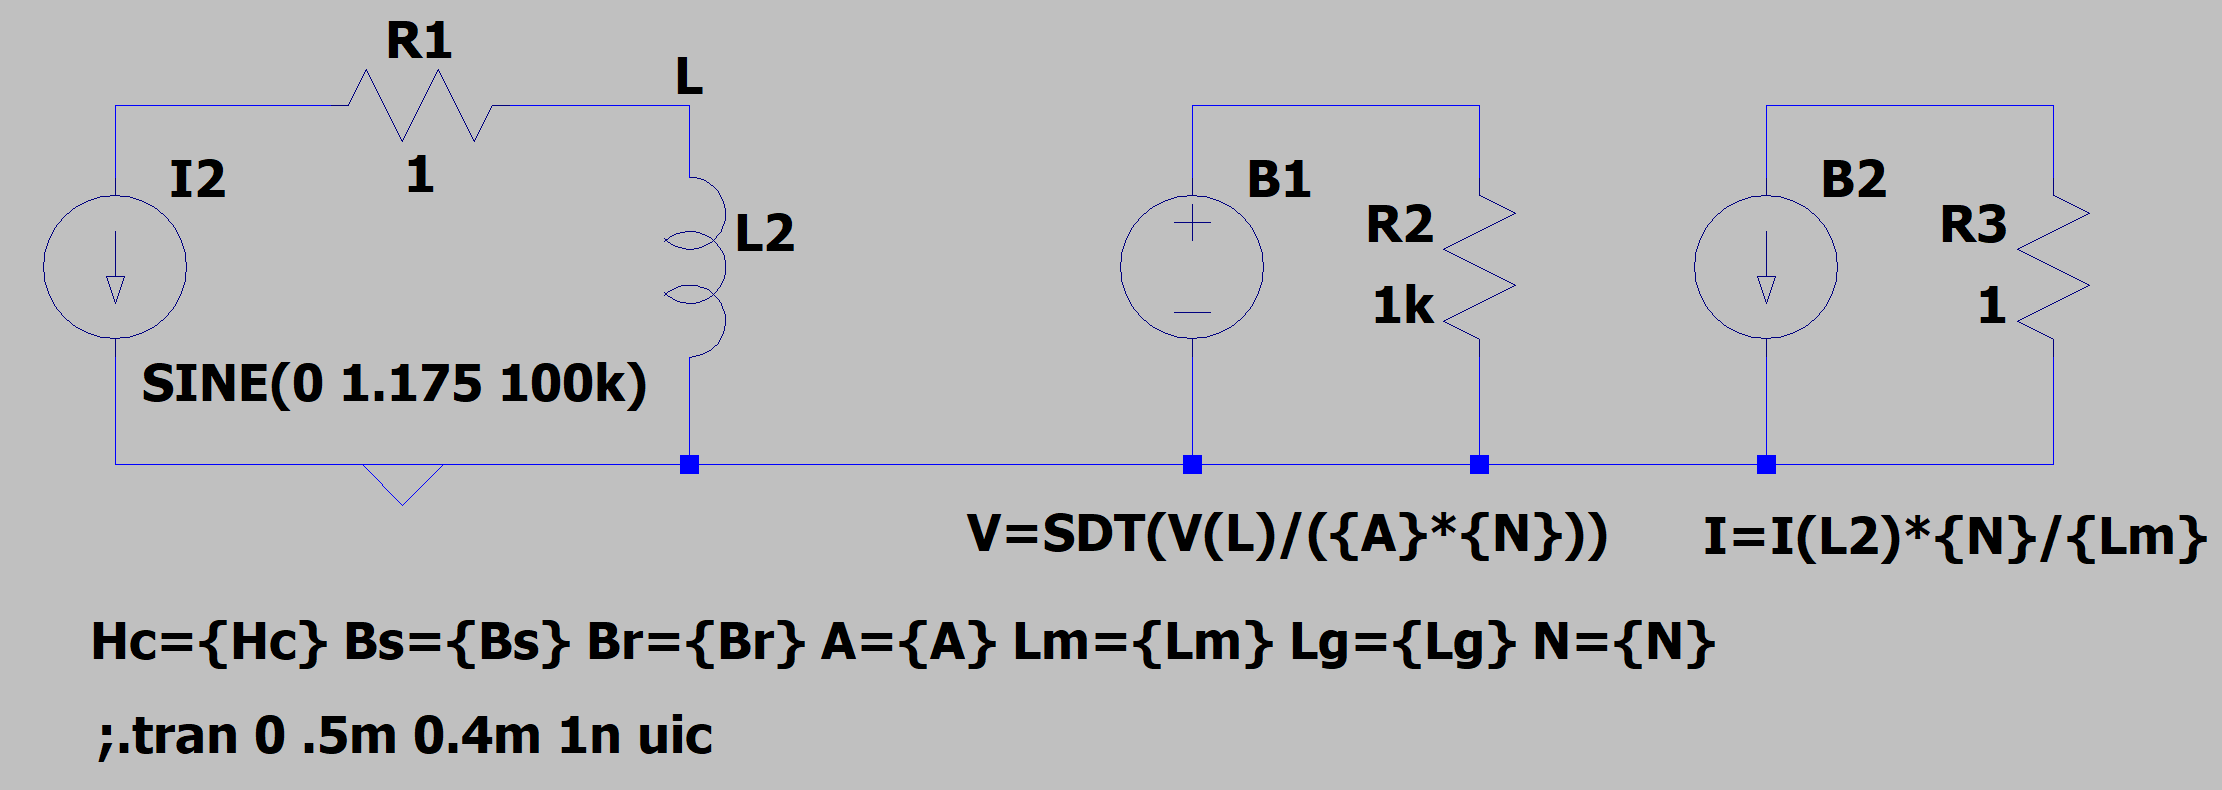
\includegraphics[width=.9\linewidth]{Bilder//Kapitel3/Hysteresis_Measurement_Setup_LTspice.png}
    \caption{Hysteresis measurement setup in LTspice}
    \label{fig:hysteresis_measurement_setup_in_LTspice}
\end{figure}
Using behavioural voltage and current sources, these equations are directly implemented in LTspice, as they allow for functions and integration.\\

Plotting the voltage of the behavioural voltage source versus the current of the behavioural current source yields the simulated B-H curve shown in figure \ref{fig:hysteresis_comparison}. The hysteresis behaviour is represented well in the simulation. While the maximum B-field $B_{max}$ does differ from the expected value by \SI{50}{\milli\tesla}, the remnant B-field $B_r$ and coercivity $H_c$ only differ minimally from the input values, by \SI{3}{\micro\tesla} and \SI{0.13}{\A\per\m} respectively.
\begin{figure}[H]
    \begin{subfigure}[b]{0.50\textwidth}
        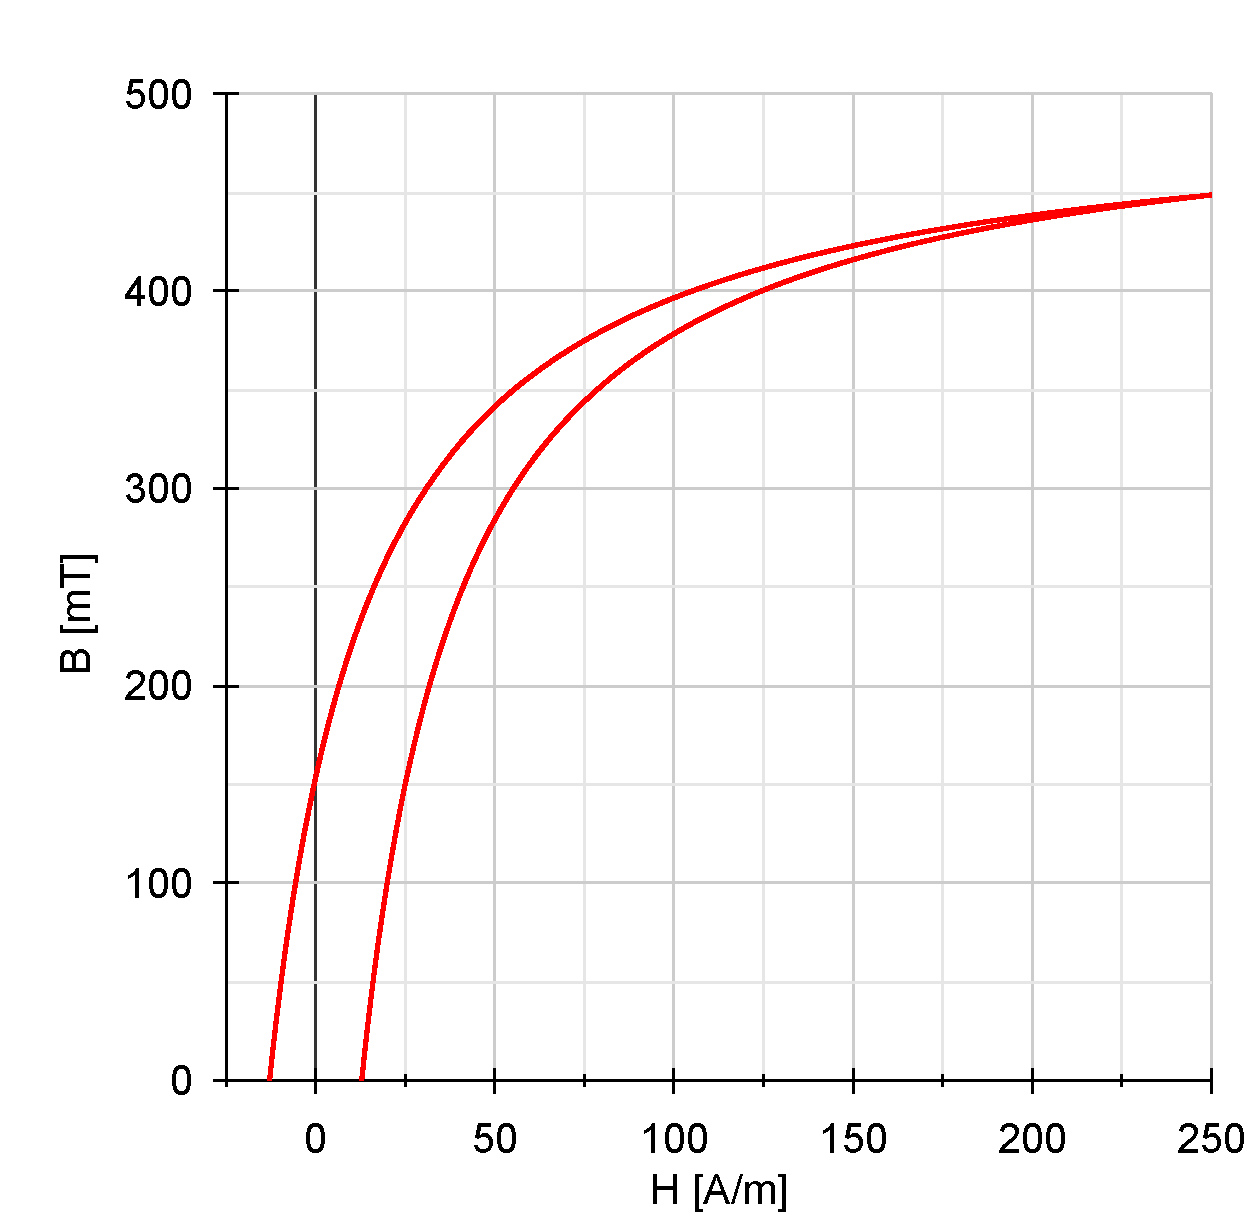
\includegraphics[width=\textwidth]{Bilder/Kapitel3/Hysteresis_LTspice_2.pdf}
        \caption{Simulated hysteresis curve}
    \end{subfigure}
    \begin{subfigure}[b]{0.49\textwidth}
        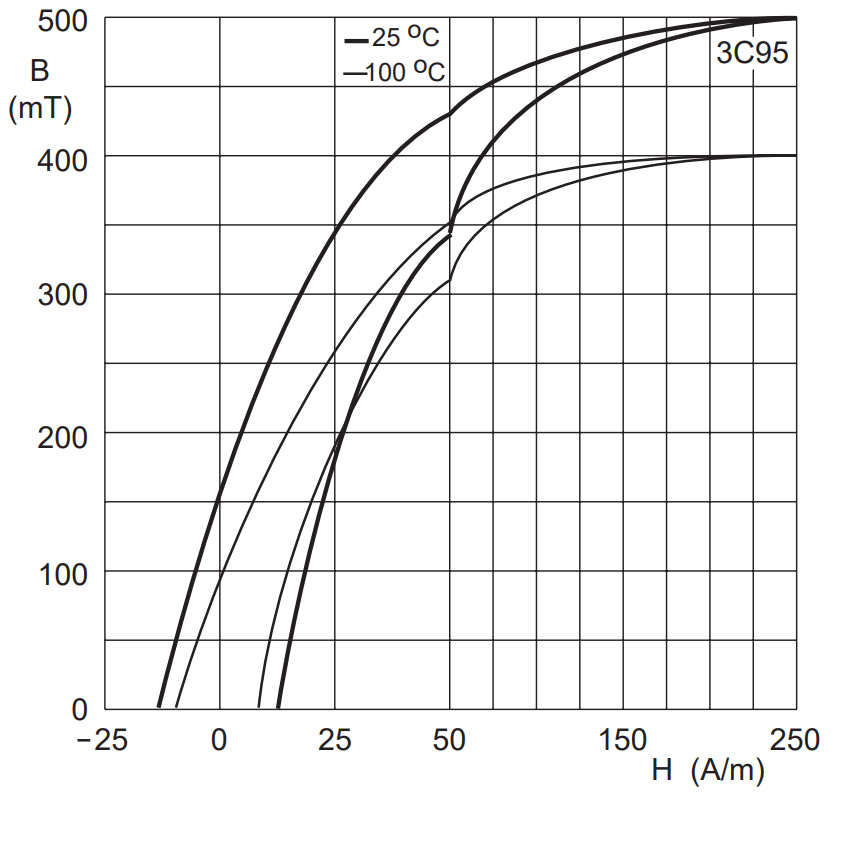
\includegraphics[width=\textwidth]{Bilder/Kapitel3/DataSheet_Hysteresis_Curve_2.png}
        \caption{Hysteresis given by the data sheet \cite{ferroxcubeProductSpecificationsCore2016}}
    \end{subfigure}
    \caption{Hysteresis comparison}
    \label{fig:hysteresis_comparison}							
\end{figure}
To validate the model's ability to function similarly to the model of section \ref{sec:modeling_the_saturation_behaviour_of_the_inductor} while adding the effects of \ac{DC} bias to the simulation, its saturation behaviour is examined. For this the measurement approach used in section \ref{sec:the_saturation_behaviour_of_the_inductor} is used again on the custom inductor. First, the physical inductor is measured and its saturation behaviour is extracted. Then the saturation of the simulated inductor model using the hysteresis parameters is measured. Their results are plotted in the graph \ref{fig:inductance_measured_and_simulatd}. 
\begin{figure}[H]
    \centering
    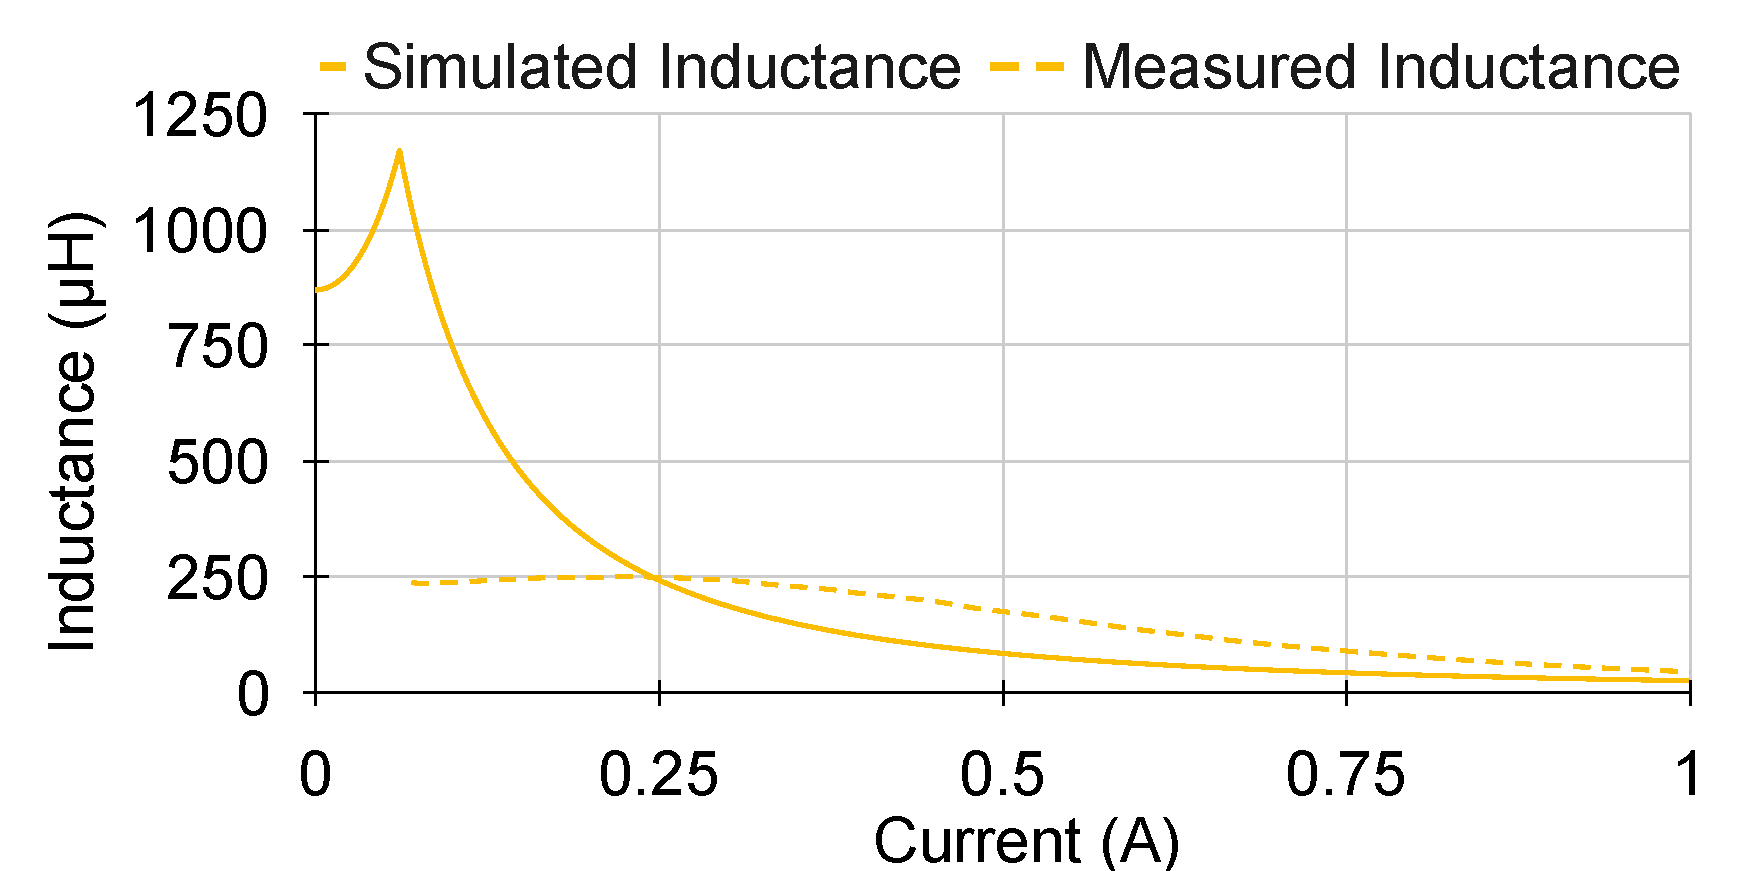
\includegraphics[width=.75\linewidth]{Bilder/Kapitel3/Saturation_Measured_and_Simulated_Hyst.pdf}
    \caption{Inductance measured and simulated}
    \label{fig:inductance_measured_and_simulatd}
\end{figure} 
Here the limits of the LTspice hysteresis modeling are shown. While demonstrating approximate hysteresis behaviour in figure \ref{fig:hysteresis_comparison}, the model is not able to recreate the inductance behaviour of the physical inductor, even though all measurement error from the hysteresis model has been removed.\\
Because of this, the hysteresis model is not implemented in the final inductor model.








\newpage
\thispagestyle{empty} 
\cleardoublepage

%/Zusammenfassung und Ausblick
% !TeX root =../main.tex
%--> SMPS, switching frequency, buck converter
%--> 3 approaches were tried, ecm, saturation, hysteresis. --> ecm and saturation worked, hysteresis didn't
%--> buck converter realised, chosen components from manufacturers
%--> realised model only able to roughly approximate ideal switching frequency. not as hoped. 
%--> Future Work: using other approaches, like behavioural sources to imitate the inductor behaviour
%-->              Using different solvers, which might yield better results
%-->              Comparison for different topologies
%-->              Proprietary solvers exist for certain inductors, modelling their behaviour in SMPS, but they aren't general / only describe the inductor
%Stellen Sie hier auf ein paar Seiten die wesentlichen Ergebnisse und Kernaussagen Ihrer Arbeit noch einmal zusammen. Sie können sehr konkret sein, da alles vorher gesagt ist. Versuchen Sie, Ihre Ergebnisse selbst zu würdigen. Seien Sie nicht zu bescheiden, machen Sie aber aus einer Mücke auch keinen Elefanten. Geben Sie Erfahrungen an, die Sie gemacht haben, die für den Leser oder nachfolgende Studierende in diesem Themenbereich möglicherweise von Interesse sein könnten. In der Zusammenfassung wird nichts Neues mehr aufgegriffen, ausgewertet oder beschrieben. Wie der Name schon sagt, werden lediglich bekannte Aspekte zusammengefasst.
%Die Arbeit sollte am Ende im Allgemeinen münden. Diese Funktion kann ein Ausblick gut übernehmen. Hierhin gehören Anregungen für eine konkrete Weiterentwicklung der Arbeit, z.B. neue Anwendungsbereiche, funktionale Erweiterungen, Modifikationen aus erkannten Problemen heraus usw., aber auch generelle Anmerkungen zur Einschätzung der zukünftigen Entwicklung der in der Arbeit behandelten Thematik.


\chapter{Summary and  Future Work} \label{sec:ausblick}
The goal of this thesis was to create an LTspice inductor model, which improves on existing models used for operations in \ac{SMPS}. This model can then be used to approximate the losses occurring in \ac{SMPS}, primarily buck converters, and help to find the ideal switching frequency to maximize efficiency. Three implementation approaches were considered based on the physical behaviour of inductors.\\
Firstly, to recreate the frequency response of the inductor an \ac{ECM} is created. Determining the frequency response was done using the "Bode 100", resulting in low noise measurements allowing for precise extraction of the inductance, capacitance and resistances of the \ac{ECM}. This model was then validated by observing its simulated frequency response, which closely matched the measured data. \\
Secondly, the saturation behaviour is included, which models the current dependent inductance of the inductor. For it a further measurement device was used, the "Power Choke Tester". Mathematical functions were matched to its output curve and imported into LTspices \textit{flux}-command. The simulated inductor was then subjected to sinusoidal currents of different amplitudes, showing how its inductance followed the desired saturation curve. To consolidate its accuracy the triangular ripple current at different \ac{DC} offsets was measured for different buck converters and compared to the simulated inductors subjected to the same load. Here the inductors however were not able to accurately recreate the ripple currents amplitude, only showing similarities in the global behaviour. While the inclusion of saturation does improve the inductor model in LTspice, it is not suited for use cases in \ac{SMPS}, inducing errors into the simulation. 
Lastly, the B-H curve of the inductor is reconstructed, to account for core losses and \ac{DC} bias. A custom inductor and measurement setup is built, to reduce the number of unknowns and capture the properties of the hysteresis curve. As the measurement is too noisy to extract precise values, 
the hysteresis curve provided by the manufacturer is used instead. With its parameters imported into LTspice, a hysteresis curve similar to the provided one can be measured. When measuring the simulated saturation behaviour of the inductor, however, it barely correlates with the measured saturation, thereby deeming this model to be unsuited for accurate \ac{SMPS} recreation.\\
After having reached the limits of the inbuilt saturation and hysteresis models of LTspice, the \ac{ECM} is tested against a physical buck converter. Making use of the provided \ac{GaNFET} models for LTspice simulation a recreation of the buck converter is implemented in LTspice. Its efficiency behaviour at different switching frequencies is compared with the physical realisation, showing a non-negligible difference between the two. The simulated efficiency approximates the behaviour of the true efficiency but is only reliably able to define a range of switching frequencies, which contains the ideal switching frequency. In conclusion, the options LTspice presents to model inductors are limited to certain use cases. While frequency response, saturation and hysteresis can all be recreated to a certain accuracy, they only represent the inductor's behaviour in certain cases and are not able to reflect accurately, how inductors in \ac{SMPS} behave.\\

The approaches used in this thesis do not exhaust the possible ways of modelling inductors with LTspice. A different approach might be to use behavioural voltage and current sources to model the effects of the \ac{DC} biased ripple current more accurately. The \ac{ECM} could also be expanded to include function-defined inductors, capacitors and resistors in an attempt to recreate the core losses. Furthermore, the different solvers of LTspice's competitors like PSpice might better reflect the inductor's behaviour in \acp{SMPS}.






\newpage
\thispagestyle{empty} 
\cleardoublepage

%|============================================================================|
%| Literaturverzeichnisse und Anhang                                          |
%|============================================================================|

%| Literaturverzeichnis 
\ifthenelse{\equal{\Sprache}{0}}
	{\bibliographystyle{StyleBib/IEEEtrans_DE.bst} % deutsches Lit.verzeichnis
	}{}
\ifthenelse{\equal{\Sprache}{1}}
	{\bibliographystyle{StyleBib/IEEEtrans_EN.bst} % englisches Lit.verzeichnis 
	}{}
\phantomsection %-> damit hyperref den Link richtig auf die erste Seite vom Literaturverzeichnis legt
% \ifthenelse{\equal{\Sprache}{0}}
% 	{\addcontentsline{toc}{chapter}{Literaturverzeichnis}
% 	}{}
% \ifthenelse{\equal{\Sprache}{1}}
% 	{\addcontentsline{toc}{chapter}{Bibliography}
% 	}{}
%\addcontentsline{toc}{chapter}{Literaturverzeichnis}
\bibliography{Literatur/literatur}

%\printbibliography	% Erzeugt die bibliographie nach den für das Package 'biblatex' definierten Kriterien
\newpage
\thispagestyle{empty}
\cleardoublepage				 

%| Anhang
%-------------

%Abbildungsverzeichnis
\listoffigures	% erstellt automatisch ein Abbildungsverzeichnis
\newpage
\thispagestyle{empty}
\cleardoublepage                                         	

% Tabellenverzeichnis
\listoftables	% erstellt automatisch ein Tabellenverzeichnis
\newpage
\thispagestyle{empty}
\cleardoublepage

\begin{appendices}
% !TeX root =../main.tex




	% Einbinden des Anhangs
\end{appendices}
\newpage
\thispagestyle{empty}
\cleardoublepage
% // Ende: Anhang //


%| Eigenständigkeitserklärung
%------------------------------

\section*{Eidesstattliche Erklärung}	% durch das sternchen taucht die eigenständigkeitserklärung nicht im inhaltsverzeichnis auf
\vspace{1cm}
\thispagestyle{empty}

Hiermit erkläre ich, \VornameDesStudenten \ \NachnameDesStudenten, dass ich die vorliegende 
        \ifthenelse{\equal{\MScBSc}{0}}
			{Bachelorarbeit}{}
		\ifthenelse{\equal{\MScBSc}{1}}
			{Projektarbeit}{}
		\ifthenelse{\equal{\MScBSc}{2}}
			{Masterarbeit}{} selbstständig und nur unter Verwendung der angegebenen Literatur und Hilfsmittel angefertigt habe. Die aus fremden Quellen direkt oder indirekt übernommenen Stellen sind als solche kenntlich gemacht. 
Die Arbeit wurde bisher in gleicher oder ähnlicher Form keiner anderen Prüfungsbehörde vorgelegt und auch nicht veröffentlicht. 
\\
\\
\par

\Ort, \today  \hfill \hrulefill

\hfill \VornameDesStudenten \ \NachnameDesStudenten \hfill

\end{document}
%|============================================================================|
%| Ende des Dokuments                                                         |
%|============================================================================|